\documentclass[twoside]{article}
\usepackage{moss} % contains layout and most imported packages.
\usepackage{cleveref}
\usepackage{amsbsy}
\usepackage{booktabs}

%%% ============================================================================
%%% Macros.
%%% ============================================================================
\DeclareMathOperator{\tr}{tr}
\DeclareMathOperator{\Tr}{Tr}
\DeclareMathOperator{\Var}{Var}
\DeclareMathOperator{\sd}{sd}
\DeclareMathOperator{\argmin}{argmin}
\DeclareMathOperator{\Cor}{Cor}
\DeclareMathOperator{\Cov}{Cov}
\DeclareMathOperator{\vvec}{vec}
\DeclareMathOperator{\vech}{vech}
\DeclareMathOperator{\w}{w}
\DeclareMathOperator{\diag}{diag} 
\DeclareMathOperator{\MSE}{MSE_Z} 
\DeclareMathOperator{\tsum}{\textstyle \sum}

\renewcommand{\sqrt}[1]{{(#1)^{1/2}}}
\newcommand\Tstrut{\rule{0pt}{2.6ex}}         % = `top' strut
\newcommand\Bstrut{\rule[-0.9ex]{0pt}{0pt}}   % = `bottom' strut

\DeclareMathOperator{\argmax}{argmax}

\title{Please avoid the standardized alpha and the ordinal alpha}

\author{
  Jonas Moss \orcid{0000-0002-6876-6964} \\
  Department of Mathematics, University of Oslo\\
  PB 1053, Blindern, NO-0316, Oslo, Norway \\
  \it{jonasmgj@math.uio.no}
}

\titletag{A PsyArXiv preprint, v1.0}
\makeatletter
\titlerunning{\@title}
\makeatother
\authorrunning{Jonas Moss}

\begin{document}
\maketitle

\begin{abstract}
Coefficient alpha is the most widely used measure of reliability. A cousin of coefficient alpha is the standardized alpha, which is calculated from the correlation matrix instead of the covariance matrix. This paper makes the case that standardized alpha should never be used. It is worse than coefficient alpha as an estimator of the congeneric reliability. There are superior estimators of the standardized reliability, and standardization should be avoided to begin with. Ordinal alpha, the standardized alpha based on the polychoric correlation matrix, should also be avoided, as it has no concrete interpretation. We propose a concrete variant of the ordinal alpha and show its relationship to the ordinal alpha.
\end{abstract}

% keywords can be removed
\keywords{reliability \and coefficient alpha \and Cronbach's alpha \and reliability of Likert scales \and factor analysis of categorical data \and ordinal alpha}

\section{Introduction}

The sample coefficient alpha is the most popular estimator of the congeneric reliability, and so it has been for a long time. A close cousin of coefficient alpha is the standardized alpha. The difference between these two alphas is easy to state: To calculate coefficient alpha you use the covariance matrix, to calculate the standardized alpha you use the correlation matrix. 

While not as popular as coefficient alpha, standardized alpha is in use. It is discussed in the popular textbook of \citet[pp. 139--141]{Furr2013-yu}, and it is readily computed using software such as SAS, SPSS, and the popular \texttt{R} \citep{Team2013-tt} package \texttt{psych} \citep{psych}. 

There are three situations where the use of standardized alpha appears to be justified. But in each situation there are alternative estimators of reliability that are demonstrably better than standardized alpha. 

\begin{enumerate}[label=(\Alph*)]

\item \textbf{The parallel model.} Standardized alpha equals the congeneric reliability under the parallel measurement model. But coefficient alpha also equals the congeneric reliability in this case. Coefficient alpha should always be preferred to standardized alpha for four reasons. (i) It is a consistent estimator of the congeneric reliability under less stringent conditions than the parallel model. (ii) It is the maximum likelihood estimator of the congeneric reliability assuming normality. (iii) It has the same asymptotic variance as standardized alpha assuming finite fourth moments. (iv) It performs about as well as standardized alpha in a small simulation study.
\item \textbf{Standardized scores.} The congeneric reliability is arguably the wrong reliability to use for standardized scores. Standardized alpha is a more reasonable choice than its direct competitor coefficient alpha since it is designed to work for standardized scores. I show there are strong reasons not to standardize your items and suggest a superior standardization method. But even if you decide to standardize your items, please avoid standardized alpha and use a plug-in estimate of the standardized reliability instead.
\item \textbf{The ordinal alpha.} A common model for Likert scale items is the normal-ogive model. In this model the covariance matrix is not identifiable, only the correlation matrix is. In this case standardized alpha can be used, but with the sample polychoric correlation matrix in place of the sample correlation matrix. This variant of standardized alpha is called the \textit{ordinal alpha} and was introduced by \citet{Zumbo2007-ap}. I argue that ordinal alpha should not be considered a proper reliability coefficient, as it has no concrete interpretation, and propose an alternative.
\end{enumerate}

The meat of the arguments are in \Cref{sec:argument A,sec:argument B,sec:Ordinal alpha}, while the next section provides background information.

%The sample coefficient alpha is by far the most popular method to measure reliability in psychology. Despite the stringent conditions that must be satisfied for its population value to be equal to the true reliability $ R$ and the questionable choice of weights $w$ \citep{McNeish2019-ea}. This has been lamented by psychometricians such as \citet{McNeish2018-vu} and \citet{Sijtsma2009-hj}. 

% But coefficient alpha is not without merits. It is easy to compute and understand \citep{Socan2000-aa}. It is well known \citep{Falk2011-ae}. It works reasonably well even when $X$ fails to be $\tau$-equivalent \citep{Raykov1997-bu}. For a recent spirited defense of coefficient alpha see \citep{Raykov2019-yr}.
%In unidimensional psychometric scales with $k$ test items, the most popular predictor $\hat{Z}$ is the sum of test items, $\hat{Z}=X_1 + \cdots + X_k$. This predictor is often called the sum score \citep{McNeish2019-ea}, and the associated reliability is the congeneric reliability \citep{Cho2016-bs}. 

% \begin{enumerate}[label=(\Alph*)]
% \item Standardized alpha and coefficient alpha are estimators of the congeneric reliability. Standardized alpha is reasonable estimator of the congeneric reliability only under the parallel model, but you should prefer coefficient alpha even if you have good reasons to believe in the parallel model. While the population values of standardized alpha and coefficient alpha equals the congeneric reliability under the parallel model, coefficient alpha equals the congeneric reliability under the more general $\tau$-equivalent model. But standardized alpha will be greater than the congeneric reliability under the $\tau$-equivalent model. Sample coefficient alpha is the maximum likelihood estimator of the congeneric reliability under the parallel model with multivariate normal errors and normal latent variables, which provides a decent heuristic argument in favor of coefficient alpha. Finally, provided the observed variables have finite fourth moments, sample coefficient alpha and sample standardized alpha have the same asymptotic variances. 

% \item A common stance on sample standardized alpha is to use it only with standardized test scores. In this case, sample standardized alpha is best understood as an estimator of the standardized reliability, i.e., the squared correlation between $Z$ and $\hat{Z}$ when $\hat{Z}$ is the sum of standardized test items. However, the standardized alpha equals the standardized reliability only under restrictive and unrealistic conditions. If you are willing to go for another kind reliability than the congeneric reliability, consider coefficient $H$ instead, which corresponds to the optimal linear predictor $\hat{Z}$. If coefficient $H$ is too hard to swallow, you can standardize with the residual errors and use the new sigma reliability.
% \end{enumerate}

%In section \ref{sec:coefficienta alpha} We introduce coefficient alpha, the standardized alpha, and the notion of reliability. We make an effort to be mathematically precise here, and reiterate several known properties about the alphas in Proposition \ref{prop:Reliabilities.}. We elaborate on argument A in section \ref{sec:argument A} and devote section \ref{sec:argument B} to argument B. In section \ref{sec:Ordinal alpha} We argue against the use of the ordinal alpha of \citet{Zumbo2007-ap} and propose an alternative.

% We end with some brief remarks in section \ref{sec:remarks}.
\section{Reliability, coefficient alpha, and standardized alpha}
\label{sec:coefficienta alpha}

Let $X$ be random variable in $\mathbb{R}^{k}$ with finite variance.
Let $\Sigma=\Cov X$ be the covariance matrix of $X$ and $\Phi=\Cor X$
be the correlation matrix of $X$. Let $\boldsymbol{1}=(1,1,\ldots,1)$ by a vector of ones of the appropriate size and $\tr$ be the trace operator.
The population coefficient alpha \citep[][eq. 2]{cronbach1951coefficient} is
\begin{equation}
\alpha =  \frac{k}{k-1}\left(1-\frac{\tr\Sigma}{\boldsymbol{1}^{T}\Sigma\boldsymbol{1}}\right)\label{eq:Coefficient alpha}
\end{equation}
and the population standardized alpha \citep[][eq. 2]{Falk2011-ae} is
\begin{equation}
\alpha_S=\frac{k}{k-1}\left(1-\frac{k}{\boldsymbol{1}^{T}\Phi\boldsymbol{1}}\right)\label{eq:standardized alpha}
\end{equation}
We care about these alphas since they sometimes coincide with the reliability coefficient under the congeneric model, a special case of the linear one-factor model. Let $Z$ be a mean zero latent variable with unit variance and $\varepsilon=(\varepsilon_{1},\varepsilon_{2},\ldots,\varepsilon_{k})$
be a mean zero vector of uncorrelated errors with unit variance. In addition, assume $Z$ and $\varepsilon$ are uncorrelated. Define the congeneric model
\begin{equation}
X=\lambda Z+\Psi^{1/2}\varepsilon,\label{eq:congeneric model}
\end{equation}
where $\lambda$ is a vector of loadings, and $\Psi^{1/2}$ is a diagonal matrix with positive diagonal elements $\sigma_i$. Since $\Psi^{1/2}$ is diagonal, the errors $\Psi^{1/2}\varepsilon$ are uncorrelated. If $\Psi^{1/2}$ is allowed to be any positive definite matrix, the model \eqref{eq:congeneric model} is a linear one-factor model, and if the dimension of $Z$ is larger than one it is a linear factor model. The random variables $Z$ and $\varepsilon$ can have any distribution whatsoever. Since $\lambda,\Psi$ are parameters of the model, we are dealing with a semi-parametric model. 

The congeneric model is most commonly used to model Likert items. But it is not is not necessarily a realistic model. The assumption of one latent factor $Z$ and the assumption of uncorrelated errors are unrealistic in most psychometric settings \citep[][Section 1.2 -- 1.3]{Green2009-le}. We restrict our attention to the congeneric model since it is commonly used, standardized alpha only makes sense on specific cases of the congeneric models, and it makes the presentation smoother. Nevertheless, the case against standardized alpha as a reliability coefficient would be even stronger in a general linear factor model. 

It is time to define reliability. Let $Z$ be an unobserved variable and $\hat{Z}$ a predictor, or measurement, of $Z$. The reliability coefficient is the squared correlation between a latent variable $Z$ and its predictor $\hat{Z}$ \citep[][p. 61]{Lord1968-ax}. 

\begin{defn}\label{defn:reliability} The reliability of $\hat{Z}$ as a predictor of $Z$ is $ R=\Cor^{2}(\hat{Z},Z)$.
\end{defn} 

The squared correlation between two variables $X$ and $Y$ quantifies the degree of linear relationship between $X$ and $Y$, with $0$ being no linear relationship and $1$ a perfect linear relationship. In the same way, the reliability coefficient quantifies how the strength of the linear relationship between $\hat{Z}$ and $Z$.

There is well-known concrete interpretation of the squared correlation as the $R^2$, or coefficient of determination. To state this relationship, we will make use of the notation $\MSE(X) = E[(X-Z)^2]$, the mean squared error of $X$ as predictor of $Z$ when $X$ is a random variable.

\begin{lem}
\label{lem:r^2 and correlation}Assume $Z$, $\hat{Z}$ have finite
variance. Then 
\begin{equation}
\Cor^{2}(\hat{Z},Z)=1-\frac{\MSE(\alpha+\beta\hat{Z})}{\Var(Z)},\label{eq:rsq and correlation}
\end{equation}
where $\alpha=E(Z)-E(\hat{Z})$ and $\beta=\Cov(\hat{Z},Z)/\Var(\hat{Z})$ are the theoretical regression coefficients minimizing the mean squared error $\MSE(\alpha+\beta\hat{Z})$. 
\end{lem}
\begin{proof}
See Appendix 1, page \pageref{proof:r^2 and correlation}.
\end{proof}

Suppose we have no predictor $\hat{Z}$ available. Then we will minimize the mean squared error by guessing $E(Z)$, and in this case $\MSE[E(Z)]=\Var(Z)$. Therefore \cref{eq:rsq and correlation} is a statement about the relative reduction in mean squared error when we use the best linear predictor based on $\hat{Z}$ instead of $E(Z)$. This interpretation of the reliability is concrete, as it numerically answers the question ``how good can I expected my best possible linear prediction of $Z$ based on $\hat{Z}$ to be?''.

In this paper the predictors $\hat{Z}$ are linear functions of $X$, that is, there are some real weights $w_{i},i=1,\ldots,k$, such that
\begin{equation}
\label{eq:Linear predictor}
\hat{Z} =  \sum_{i=1}^{k} w_{i}X_i = \sum_{i=1}^{k}w_{i}(Z\lambda_i + \sigma_{i} \varepsilon_i).\nonumber 
\end{equation}
The second equation follows from the definition of $X$ in the congeneric model \eqref{eq:congeneric model}. 

In this proposition, and the rest of the paper, we will use the notation $\overline{x}$ to denote the mean of the vector $x$. Moreover, when $x$ and $y$ are vectors of the same length, $xy$ is the pointwise product of $x$ and $y$.

\begin{prop}
\label{prop:reliability motivation}Assume the congeneric model \eqref{eq:congeneric model}. Let $\hat{Z}=\sum_{i=1}^{k}w_{i}X$
for some vector of weights $w$ with elements $w_{i},i=1,\ldots,k$. Then the reliability equals
\begin{eqnarray}
 R_w & = & \frac{(w^{T}\lambda)^{2}}{(w^{T}\lambda)^{2}+w^{T}\Psi w}\label{eq:linear reliabiltiy}\\
 & = & 1- \MSE (w_{0}\hat{Z})\label{eq:MSE}
\end{eqnarray}
where $\MSE (w_{0}\hat{Z})=E[(Z-w_{0}\hat{Z})^{2}]$ is the
mean squared error, $w_{0}=\overline{w\lambda}/(k\overline{w\lambda}^{2}+\overline{w^{2}\sigma^{2}})$ is the constant minimizing the mean squared error.
\end{prop}
\begin{proof}
See Appendix 1, page \pageref{proof:reliability motivation} for a proof.
\end{proof}

Equation \eqref{eq:linear reliabiltiy} is the definition \citet[][p. 112]{Joreskog1971-nn} gave of the composite reliability under the congeneric model \eqref{eq:congeneric model}. 
The role of $w_0$ in Proposition \ref{prop:reliability motivation} is to make sure $\hat{Z}$ predicts $Z$ on he right scale, and in this paper the scale of $Z$ is fixed by $\Var Z = 1$. Since $Z$ is latent we would usually not care about this scale, but it is handy to fix it to $1$ since it allows us to compare different predictors of $\hat{Z}$. The formulation $1-\MSE (w_{0}\hat{Z})$ is more concrete than the correlation formulation, as it explicitly references the predictor $w_{0}\hat{Z}$, while the correlation is scale-free and more abstract. The mean squared error definition is amenable to generalizations as well.

A modestly popular choice for $w$ are the weights minimizing the mean squared error, known as the Thurstone weights \citep{thurshronebook}, $w_{i}=\lambda_{i}/[\sigma_{i}^{2}(1+k\overline{\lambda^{2}\sigma^{-2}})],\:i=1,\ldots,k$. Using these weights lead to coefficient $H$ \citep{hancock2001rethinking}, also known as the maximal reliability \citep{Li1997-yh}, 
\begin{equation}
\label{eq:coefficient_H}
 R_{H}=\frac{k\overline{\lambda^{2}\sigma^{-2}}}{k\overline{\lambda^{2}\sigma^{-2}}+1},
\end{equation}
where $\overline{\lambda^{2}\sigma^{-2}} = k^{-1}\sum_{i=1}^{k}\lambda_{i}^2/\sigma_i^2$. By \cref{prop:reliability motivation}, the weights are equivalent to $w_i = \lambda_i/\sigma_i^2$ and $w_0 = \sigma_{i}^{2}(1+k\overline{\lambda^{2}\sigma^{-2}})$, which are much easier to interpret.

By far the most popular choice is to give the same weight to each $X_i$, that is, $w = \boldsymbol{1}=(1,1,\ldots,1)$. This leads to the congeneric reliability, which is the estimand of coefficient alpha under certain conditions. Its definition is
\begin{equation}
 R =\frac{k\overline{\lambda}^{2}/\overline{\sigma^{2}}}{k\overline{\lambda}^{2}/\overline{\sigma^{2}} + 1}\label{eq:Congeneric reliability}
\end{equation}
where $\overline{\lambda}=k^{-1}\sum_{i=1}^{k}\lambda_{i}$ and
$\overline{\sigma^{2}}=k^{-1}\sum_{i=1}^{k}\sigma_{i}^{2}$. 

Finally, the weights $w_i = (\lambda_i^2 + \sigma_i^2)^{-1/2}$ yield the standardized reliability. The standardized reliability is the estimand of the standardized alpha under the certain conditions, and can be written as
\begin{equation}
 R_S=\frac{k\overline{\lambda(\lambda^{2}+\sigma^{2})^{-1/2}}^{2}/\overline{\sigma^{2}(\lambda^{2}+\sigma^{2})^{-1}}}{k\overline{\lambda(\lambda^{2}+\sigma^{2})^{-1/2}}^{2}/\overline{\sigma^{2}(\lambda^{2}+\sigma^{2})^{-1}}+1}.\label{eq:Standardized reliability}
\end{equation}

\cref{prop:reliability motivation} connects all reliabilities on the form of \cref{eq:Linear predictor} to their unique optimal predictor $\hat{Z}$. Given a vector of weights $w$, the only linear predictor minimizing the mean squared error $\MSE(\hat{Z})$ while simultaneously satisfying $1-\MSE(\hat{Z})=R_w$ is $\hat{Z}=w_0\sum_{i=1}^k w_iX_i$. This relationship also holds for the well-known reliabilities in \cref{eq:coefficient_H,eq:Congeneric reliability,eq:Standardized reliability}.

There is a well-known relationship between the congeneric reliability and coefficient alpha. This relationship can be generalized to weighted reliabilities. Define the generalization of the coefficient alpha and the standardized alpha, the \textit{weighted alpha},

\begin{defn}
Let $w$ be a vector of weights and $\Sigma$ a covariance matrix. The \textit{weighted alpha} is
\begin{equation}
\alpha_{w}=\frac{k}{k-1}\left(1-\frac{w^{T}(\diag\Sigma)w}{w^{T}\Sigma w}\right)\label{eq:weighted alpha}
\end{equation}
where $\diag\Sigma$ is the diagonal matrix with diagonal equal to the diagonal of $\Sigma$.
\end{defn}
The ordinary coefficient alpha \eqref{eq:Coefficient alpha} has weights $w=\boldsymbol{1}$
while the standardized alpha \eqref{eq:standardized alpha} has weights $w_{i}=\sqrt{\lambda_{i}^{2}+\sigma_{i}^{2}}$. Coefficient alpha and standardized alpha are the most interesting cases of the weighted alpha, as you can calculate them using only the covariance matrix $\Sigma = \Cov X$. When $w$ are for instance the Thurstone weights, $a_w$ is not a function of $\Sigma$, as they require knowledge of the factor loadings $\lambda$ and the residual errors $\sigma$. Still, the definition makes sense for any weight $w$. 

The following proposition summarizes the basic relationship
between the reliability $ R_{w}$ and the weighted $\alpha_{w}$. To state it, we will need
the notion of a \textit{$\tau$-equivalent model} \citep[][section 2.13]{Lord1968-ax}. A congeneric model \eqref{eq:congeneric model} is \textit{$\tau$-equivalent} if $\lambda_{i}=\lambda_{j}$ for all $i,j$. That is, all unstandardized
factor loadings are equal.
\begin{prop}
\label{prop:weighted alpha}Let $w$ be a vector of weights and
assume $X$ follows the congeneric model \eqref{eq:congeneric model}. Then 
\begin{equation}
\alpha_{w}= R_{w}-\frac{k}{k-1}\frac{\overline{w^{2}\lambda^{2}}-\overline{w\lambda}^{2}}{k\overline{w\lambda}^{2}+\overline{w^{2}\sigma^{2}}}\label{eq:alpha-omega discrepancy}
\end{equation}
and $\alpha_w \leq  R_w$ with equality if and only if $wX$ is $\tau$-equivalent, i.e. $w_i\lambda_{i}=w_j\lambda_{j}$
for all $i,j$.
\end{prop}
\begin{proof}
See Appendix 1, page \pageref{proof:weighted alpha}
for a proof. The inequality $\alpha\leq R$ is classical \citep[][Theorem 4.4.3]{Lord1968-ax}. The discrepancy term in \eqref{eq:alpha-omega discrepancy} for the special case of coefficient alpha is extensively discussed by \citet{Raykov1997-bu}. 
\end{proof}

% By Chebyshev's inequality, $k\overline{w\lambda}^{2}\geq\overline{(w\lambda)^{2}}$,
% with equality if and only if $w_{i}\lambda_{i}=w_{j}\lambda_{j}$,
% that is, the weighted model is $\tau$-equivalent. The discrepancy term in \eqref{eq:alpha-omega discrepancy} for the special case of coefficient alpha is extensively discussed by \citet{Raykov1997-bu}. 

Proposition \ref{prop:weighted alpha} is a minor generalization of the two most frequently mentioned fact about coefficient alpha: (i) That $\alpha =  R$ under the $\tau$-equivalent model. (ii) Coefficient alpha is a lower bound for the congeneric reliability (that is, $\alpha \leq  R$) under the congeneric model.
 
When $w_{i}=\sqrt{\lambda_{i}^{2}+\sigma_{i}^{2}}$, $wX$ is $\tau$-equivalent if and only if the standardized factor loadings are equal, and Proposition \ref{prop:weighted alpha} tells us that standardized alpha equals the standardized reliabiltiy (that is, $\alpha_S =  R_S$) in this case. 

The next proposition explores the relationship between coefficient alpha, the standardized alpha, and the congeneric reliability coefficient.

\begin{prop}
\label{prop:Reliabilities.}Assume the congeneric model \eqref{eq:congeneric model}. Let $\alpha$ be coefficient alpha \eqref{eq:Coefficient alpha}, $\alpha_S$ be the standardized alpha \eqref{eq:standardized alpha}, and  $ R$ be the congeneric reliability \eqref{eq:Congeneric reliability}. 
\begin{enumerate}[label=(\roman*)]
\item Assume $\lambda_{i}=\lambda_{j}$ for all $i,j$, i.e. the $\tau$-equivalent model. Then $\alpha_S \geq \alpha =  R$, with equality if and only if $\sigma_{i}=\sigma_{j}$ for all $i,j$ or $\lambda_i = 0$ for all $i$.
\item If $k=2$, $\alpha_S\geq\alpha$, with equality if and only if $\lambda_{1}^{2}+\sigma_{1}^{2}=\lambda_{2}^{2}+\sigma_{2}^{2}$ or $\lambda_1 = 0$ or $\lambda_2 = 0$. But if $k>2$, both $\alpha_S>\alpha$
and $\alpha_S<\alpha$ are possible.
\item All of $\alpha_S= R$, $\alpha_S> R$ and $\alpha_S< R$
are possible when $\lambda_{i}\neq\lambda_{j}$ for some $j$. In particular, $\alpha_S \geq  R$ when $\lambda_i = \sigma_i$ for all $i$, and $\alpha_S \leq  R$ when $\lambda_i^2 + \sigma_i^2$ is constant. Both inequalities are equalities if and only if all $\lambda$s are equal.
\end{enumerate}
\end{prop}
\begin{proof}
See page \pageref{proof:Reliabilities.} of Appendix 1 for a proof.
\end{proof}

A congeneric model satisfying $\sigma_{i}=\sigma_{j}$ for all $i,j$ is called a \textit{parallel model} \citep[][section 2.13]{Lord1968-ax}. 

That $\alpha = R$ under the $\tau$-equivalent model and $\alpha_S = R$ under the parallel model show us a way to estimate the congeneric reliability $R$ using a simple function of the sample covariance $S$. The intuitive estimate of $R$ is the plug-in estimator, which needs estimates of $\lambda$ and $\sigma$. But to estimate these we need to use iterative algorithms and complex software. That $\alpha_S$ and $\alpha$ are easy to calculate is barely an advantage these days though, as it is easy to estimate $\lambda$ and $\sigma$ using for instance the \texttt{R} \citep{Team2013-tt} package \texttt{lavaan} \citep{Rosseel2012-yg}. Estimating $R$ using the plug-in estimator allows us to forego the unrealistic assumptions of $\tau$-equivalence and parallel test items altogether, and is recommended by e.g. \citet{McNeish2019-ea}.

%\begin{rem}
%We do not have to assume normality or continuous $X$s to get Proposition \ref{prop:weighted alpha}. The derivations in Proposition \ref{prop:weighted alpha} uses no assumptions about the distributions of $Z$ and $\varepsilon$ except that they have finite second moments. This is contrary to some claims about coefficient alpha made by, e.g. \citet[][p.415]{McNeish2018-vu}, \citet[][p.21]{Zumbo2007-ap} and \citet[][p. 1185]{Zumbo2019-lm}. \citet{Raykov2019-yr} lamented this widespread misunderstanding, while \citet[][p. 1060]{Chalmers2018-fj} investigated the source of the misunderstanding. That said, while continuous data is no assumption for the coefficient alpha or the congeneric reliability, the implicitly assumed congeneric model \eqref{eq:congeneric model} is unrealistic for discrete data. 
%\end{rem}
\begin{rem}
While $\alpha_S$ is an upper bound for $\alpha$ when $k = 2$ and under the $\tau$-equivalent model, it does not bound $\alpha$ in either direction otherwise, see Proposition \ref{prop:Reliabilities.}. This is contrary to claims in the literature such as that of \citet[][p.348]{Osburn2000-jd} \enquote{When the components of a composite measure are congeneric, standardized alpha will always exceed the true reliability}. \citet[][p.450]{Falk2011-ae} has a clearly laid out example of $\alpha>\alpha_S$.
\end{rem}

%  The Open Science Foundation repository for this paper (\url{https://osf.io/s356h/}) contains code to generate parameter value $\lambda,\sigma$ such that $\alpha_S =  R$.

By Proposition \ref{prop:weighted alpha}, coefficient alpha equals the congeneric reliability if and only if all the factor loadings $\lambda$ are equal. But there is no simple necessary and sufficient criterion for $\alpha_S =  R$, as Proposition \ref{prop:weighted alpha} (ii) entails that the parallel model is merely sufficient. Still, these cases are like lucky coincidences, and it would be preposterous to assume $\alpha_S =  R$ for unknown parameter values without assuming the parallel model.

Let us proceed to the sample variants of coefficient alpha and standardized
alpha. Let $S$ be a sample covariance matrix based on
$n$ samples of $X$ and $P$ the sample correlation matrix.
The sample coefficient alpha is 
\begin{equation}
\hat{\alpha}=\frac{k}{k-1}\left(1-\frac{\tr{S}}{\boldsymbol{1}^{T}S\boldsymbol{1}}\right)\label{eq:sample coefficient alpha}
\end{equation}
while the sample standardized alpha is
\begin{equation}
\hat{\alpha}_s=\frac{k}{k-1}\left(1-\frac{k}{\boldsymbol{1}^{T}P\boldsymbol{1}}\right)\label{eq:sample standardized alpha}
\end{equation}
The congeneric reliability \eqref{eq:Congeneric reliability} has no
simple sample version, as it depends on estimates of $\lambda$ and
$\sigma^2$, which usually do not have closed forms.

\section{Situation A. The parallel model}
\label{sec:argument A}

How does sample coefficient alpha \eqref{eq:sample coefficient alpha} compare to sample standardized alpha \eqref{eq:sample standardized alpha} as estimators of the congeneric reliability \eqref{eq:Congeneric reliability}? From Proposition \ref{prop:Reliabilities.} we know the parallel model is the natural setting to make comparisons, as this is the only case when coefficient alpha and the standardized alpha equals the congeneric reliability with certainty.

The parallel model is
\begin{equation}
\label{eq:parallel model}
X = \lambda Z + \sigma\varepsilon,
\end{equation}
where $\lambda$ and $\sigma$ are positive scalars and $\varepsilon\in\mathbb{R}^k$ and $Z\in\mathbb{R}$ are uncorrelated random variables with unit variance and zero mean. Model \eqref{eq:parallel model} is clearly a special case of the congeneric model \eqref{eq:congeneric model}. Our goal is to estimate the congeneric reliability \eqref{eq:Congeneric reliability}, which for the parallel model equals
\begin{equation}
\label{eq:parallel_omega}
 R = \frac{k\lambda^2/\sigma^2}{k\lambda^2/\sigma^2 + 1}.
\end{equation}
Now we have a model, a parameter, and two competing estimators of that parameter, namely $\hat{\alpha}$ and $\hat{\alpha}_s$. Which should we choose? 

Choosing between estimators is a classical statistical problem. Some well-established methods to approach such problems are:

% Let $\rho = \lambda^2/\sqrt{\lambda^2 + \sigma^2}$ be the unique off-diagonal correlation of $\Cor(x)$. 

\begin{enumerate}[label=(\Alph*)]
\item Check the relative asymptotic efficiency of the estimators.
\item Is any of the competing estimators a maximum likelihood estimator under the appropriate parametric restrictions?
\item Compare finite-sample performance of the estimators in terms of for instance mean squared error.
\item Investigate the robustness of the estimators against misspecification of the model.
\end{enumerate}

Point (D) about robustness is an easy one, as we have already established that coefficient alpha is more robust than the standardized alpha. For by Proposition \ref{prop:Reliabilities.}, coefficient alpha equals the congeneric reliability under the $\tau$-equivalent model and standardized alpha does not. Thus we can check (D) off our list as an easy win for coefficient alpha.

\subsection{Maximum likelihood}
In this section we will work with the parallel model \eqref{eq:parallel model} where $Z$ and $\varepsilon$ are independent standard normals. Call this model the normal parallel model.

Coefficient alpha the maximum likelihood estimator of $ R$ in the normal parallel model provided it is non-negative, see Theorem \ref{thm:ML} below for details. Why does this matter? For one thing, maximum likelihood estimators are guaranteed to be efficient under quite weak conditions \citep[][Section 7.3]{Lehmann2004-ke}. But maximum likelihood also has an heuristic justification; maximizing likelihood is an intuitive procedure and is the most popular recipe for making estimators.

\begin{thm}\label{thm:ML}
Assume the normal parallel model.
\begin{enumerate}[label=(\roman*)]
\item The maximum likelihood estimates of $\lambda^{2}$
and $\sigma^{2}$ are 
\begin{eqnarray*}
\hat{\lambda}^2_\textrm{ML} & = & \begin{cases}
\frac{1}{(k-1)k}(\boldsymbol{1}^{T}S\boldsymbol{1}-\tr{S}) & \boldsymbol{1}^{T}S\boldsymbol{1}\geq\tr{S},\\
0 & \text{\textrm{otherwise}},
\end{cases}\\
\end{eqnarray*}
and
\begin{eqnarray*}
\hat{\sigma}^2_\textrm{ML} & = & \begin{cases}
\frac{1}{k-1}(\tr{S}-\boldsymbol{1}^{T}S\boldsymbol{1}/k) & \boldsymbol{1}^{T}S\boldsymbol{1}\geq\tr{S},\\
\frac{\tr{S}}{k} & \textrm{otherwise}.
\end{cases}
\end{eqnarray*}
\item The maximum likelihood estimator of the congeneric reliability
\eqref{eq:Congeneric reliability} equals the sample coefficient alpha
when $\boldsymbol{1}^{T}S\boldsymbol{1}\geq\tr{S}$ and $0$ otherwise. That is,
\begin{eqnarray*}
\hat{ R}_\textrm{ML} & = & \begin{cases}
\hat{\alpha} & \boldsymbol{1}^{T}S\boldsymbol{1}\geq\tr{S},\\
0 & \text{\textrm{otherwise}}.
\end{cases}
\end{eqnarray*}
\end{enumerate}
\end{thm}
\begin{proof}
See page \pageref{proof:ML} of Appendix 1 for a proof. 
\end{proof}

\subsection{Asymptotic efficiency}
Comparing efficiencies is the most popular method to compare estimators. Let $\hat{\theta}_1$ and $\hat{\theta}_2$ be two estimators converging at the $n^{1/2}$-rate to normal distributions centered on the same parameter $\theta$. The asymptotic variance of the first distribution is $\phi_1^2$ and the asymptotic variance of the second distribution is $\phi_2^2$. Then $\theta_1$ is more efficient than $\theta_2$ if $\phi_1<\phi_2$. 

An estimator $\hat{\theta}$ is \textit{efficient} \citep[][Section 4.3]{Lehmann2004-ke} if its asymptotic variance is smaller than any other estimator. Maximum likelihood estimators are efficient under weak conditions, hence $\alpha$ is efficient under the normal parallel model by Theorem \ref{thm:ML}.  

\begin{thm}
\label{thm:asymptotics}
Assume $X$ has finite variance. 
\begin{enumerate}[label=(\roman*)]
    \item Both sample coefficient alpha and sample standardized alpha converge to their population counterparts with probability $1$. Under the parallel model they are strongly consistent and converge to the congeneric reliability. That is, $\hat{\alpha}\to\alpha$ and $\hat{\alpha}_s\to\alpha_S$ with probability $1$ and $\alpha = \alpha_S =  R$.
    \item Under the parallel model \eqref{eq:parallel model}, coefficient alpha and standardized alpha share a normal limit distribution when $Z$ and $\varepsilon$ have finite fourth moments, i.e. $n^{1/2}(\hat{\alpha} - \alpha)$ and  $n^{1/2}(\hat{\alpha}_s - \alpha_S)$ both converge to the same normal variable $Z$.
    \item Under the normal parallel model, both $\alpha$ and $\alpha_S$ are efficient. Their common limit is normal with asymptotic variance 
    $$\sigma^{2}(\alpha)= \sigma^{2}(\alpha_S)=2\frac{k}{k-1}(1-\alpha_S)^{2}.$$
\end{enumerate}
\end{thm}    
\begin{proof}
See page \pageref{proof:asymptotics} of Appendix 1 for a proof of (i) and (iii). Appendix 2 (p. \pageref{Appendix 2}) contains the proof of (ii) together with an expression of the common variance. The proof of (ii) relies heavily on the work of \citet{Van_Zyl2000-si} and \citet{hayashi2005note}. The proof of (iii) relies on \citet[][eq. 13]{Van_Zyl2000-si} and \citet[][eq. 58]{Kristof1963-tb}, who, among others, derived the limit distribution of coefficient alpha under the normal parallel model.
\end{proof}

\begin{rem}
Item (i) states that both $\hat{\alpha}_s$ and $\hat{\alpha}$ estimate what they should. \citet{Raykov2019-tv} is an introduction to convergence with probability $1$ in the psychometry context and contains a proof of (i) for coefficient alpha. Item (ii) is the main argument of this section. It shows that $\hat{\alpha}_{s}$ and $\hat{\alpha}$ will perform equally well in the limit. It does not matter what $\lambda$, $\sigma$ and the distributions of $Z$, $\varepsilon$ are; we only require that the models have finite fourth moments. Regarding item (iii), a straightforward consequence of Theorem \ref{thm:ML} is that $\hat{\alpha}$ is efficient under the normal parallel model, and in this sense (iii) is an extension of said theorem. The shared limit distribution is simple enough to be usable in practice.
\end{rem}

\subsection{A small simulation}
There is no reason to choose standardized alpha over coefficient alpha from an efficiency standpoint. But it might still be the case
that the standardized alpha outperforms coefficient alpha
in small samples. This section contains a small simulation
study comparing the mean squared error of the estimators under
the parallel model. Since the coefficient alpha is the maximum likelihood
estimator for the normal parallel model there is a heuristic reason
to believe it will perform better than the standardized estimator
in this context. Instead of normal errors, we will use three non-normal
errors:

\begin{enumerate}
\item Scaled $t$-distribution with $5$ degrees of freedom. The $t$-distribution
has heavier tails than the normal distribution but is symmetric and nearly bell-shaped. 
\item Scaled and centered Beta distribution with $\alpha=\beta=1/10$. This is a bimodal distribution with much weight placed on the modes at $0$ and $1$. 
\item Scaled and centered Gamma distribution with $\alpha=\beta=1/100$. This is asymmetric and with heavy tails. 
\end{enumerate}

All of the distributions are extreme, and should be able to force out the difference between the estimators. We use $5$ degrees of freedom for the $t$-distribution since it is the first integer degree of freedom where $t$ has finite fourth moment. The Open Science Foundation repository for this paper (\url{https://osf.io/s356h/}) contains the code for the simulations.

%% <<<<< Example table start (\label{tab:reliabilites})
% latex table generated in R 3.6.2 by xtable 1.8-4 package
% Mon Feb 03 15:19:37 2020
\begin{table}[ht]
\centering
\caption{Simulations of $100 \times \textrm{MSE}_\alpha/\textrm{MSE}_{\alpha_s}$ in the parallel model} 
\begin{tabular}{rlllllllll}
    & $t(5)$ & $t(5)$ & $t(5)$ & Beta & Beta & Beta & Gamma & Gamma & Gamma \\
  & $\sigma = 2$ & $\sigma = 1$ & $\sigma = 0.5$ & $\sigma = 2$ & $\sigma = 1$ & $\sigma = 0.5$ & $\sigma = 2$ & $\sigma = 1$ & $\sigma = 0.5$ \\
$k = 5, n = 50$ & 106 & 112 & 103 & 106 & 112 & 114 & 107 & 105 & 113 \\ 
  $k = 20, n = 50$ & 113 & 105 & 105 & 95.8 & 90.8 & 98.9 & 97.5 & 97.6 & 94.7 \\ 
  $k = 5, n = 200$ & 99.5 & 98.7 & 102 & 101 & 101 & 100 & 74.7 & 60.6 & 67.4 \\ 
  $k = 20, n = 200$ & 37.8 & 174 & 138 & 144 & 82.6 & 308 & 257 & 189 & 153 \\ 
  \end{tabular}
\end{table}
\newcommand{\geomean}{1.08}


%% example table end >>>>>

Table \ref{tab:simulation} contains $100 \times \MSE(\alpha)/\MSE(\alpha_S)$, where $\MSE$ denotes the mean squared error. Values higher than $100$ are in favor of $\hat{\alpha}_S$ and values lower than $100$ in favor of $\hat{\alpha}$. The table shows that $\alpha_S$ tends to outperform $\alpha$ when both $k$ and $n$ are large and $\sigma$ is small, but with no clear trends otherwise. In this simulation $\hat{\alpha}_s$ does slightly better than $\hat{\alpha}$ -- the geometric mean of $\MSE(\alpha)/\MSE({\alpha_S})$ is $1.08$, giving an $8$\% advantage to $\hat{\alpha}_s$. Of course, this is a small simulation study and it is hard to predict what would happen with other distributions. Still, the result of these simulations should be counted in favor of sample standardized alpha.

To sum up, sample alpha won the maximum likelihood and robustness competitions, drew the asymptotic efficiency competition, and lost the finite sample competition. The tally is coefficient alpha 2\sfrac{1}{2} - 1\sfrac{1}{2} standardized alpha. 

\section{Situation B. Standardized scores}
\label{sec:argument B}

Standardized alpha is explicitly linked to the standardized reliability \eqref{eq:Standardized reliability} but not to the congeneric reliability \eqref{eq:Congeneric reliability}. Recall the definition of reliability from
\Cref{sec:coefficienta alpha}. Given a predictor $\hat{Z}$ of $Z$, the
reliability $ R$ equals the square correlation between $\hat{Z}$
and $Z$, or $ R=\Cor^{2}(\hat{Z},Z)$. Assume
we know the values of $\lambda$ and $\sigma$. When we use unstandardized
scores, our predictor is 
\begin{equation}
\hat{Z}=w_{0}\sum_{i=1}^{k}X_{i}\label{eq:sum score}
\end{equation}
where $w_{0}=\overline{\lambda}/(k\overline{\lambda}^{2}+\overline{\sigma^{2}})$ scales the predictions to match $\Var Z=1$ (recall Proposition \ref{prop:reliability motivation}). When we use standardized
scores, our predictor is
\begin{equation}
\hat{Z}^{*}=w_{0}\sum_{i=1}^{k}(\lambda^{2}+\sigma^{2})^{-1/2}X_{i}\label{eq:standardized sum score}
\end{equation}
These predictors are not the same in general, and their reliabilities are not
the same either.

This difference matters. Reliability coefficients are useful because they tell you how good you can expected your prediction of $Z$ based on $X$ to be. Provided you use the mean squared error as a measure of prediction success, this is exactly what the mean squared error-based reliability concept in Proposition \ref{prop:reliability motivation} says. For $1 - \MSE(w_0\hat{Z})$ puts a number between $0$ and $1$ on the expected quality of your prediction. If you do not use the predictor $\hat{Z}$, but some other predictor $\hat{Z}'$, this concrete interpretation of the reliability disappears. 

An important motivation for using the squared
correlation between $Z$ and $\hat{Z}$ as the definition of a
reliability coefficient is that it allows us to do correction for
attenuation. Let $\hat{Z}_{1},\hat{Z}_{2}$ be two linear
predictors of two latent variables $Z_{1},Z_{2}$ defined on two separate
congeneric models. Assume the errors $\varepsilon_{1}$ and $\varepsilon_{2}$ of these models
are uncorrelated. Our goal is to find the correlation $\Cor(Z_{1},Z_{2})$
between the latent variables $Z_{1}$ and $Z_{2}$ using only the
reliabilities $ R(\hat{Z}_{1})$, $ R(\hat{Z}_{2})$,
and the observed correlation $\Cor(\hat{Z}_{1},\hat{Z}_{2})$.
Then
\begin{eqnarray*}
\Cor(\hat{Z}_{1},\hat{Z}_{2}) & = & \frac{\Cov(Z_{1},\hat{Z}_{1})\Cov(Z_{2},\hat{Z}_{2})}{\sd(\hat{Z}_{1})\sd(\hat{Z}_{2})}\Cor(Z_{1},Z_{2}),\\
 & = & \sqrt{ R(\hat{Z}_{1})}\sqrt{ R(\hat{Z}_{2})}\Cor(Z_{1},Z_{2}),
\end{eqnarray*}
and $\Cor(Z_{1},Z_{2})=\Cor(\hat{Z}_{1},\hat{Z}_{2})/\sqrt{ R(\hat{Z}_{1}) R(\hat{Z}_{2})}$,
the famous \citet{spearman1904proof} attenuation formula.

%Correction for attenuation cannot be used unless both $ R(\hat{Z}_i)$s are the squared correlation between $\hat{Z}_i$ and $Z_i$. For example,

Assume you use the standardized sum scores $\hat{Z}_1^*$, a predictor on the form of  \cref{eq:standardized sum score}, to make predictions for $Z_1$. To predict $Z_2$ you use the $\hat{Z}_2$, a predictor on the form of \cref{eq:sum score}. Then the correlation between your predictions is $\Cov(\hat{Z}_1^*,\hat{Z}_2)$. Now it would be wrong to use the congeneric reliability for $Z_1$ in Spearman's formula, as it based on the sum scores $\hat{Z}_1$. If you used the congeneric reliability, the correlation between $Z_1$ and $Z_2$ would incorrectly be calculated according to $\Cor(\hat{Z}_{1}^*,\hat{Z}_{2})= \sqrt{ R(\hat{Z}_{1}) R(\hat{Z}_{2})}\Cor(Z_{1},Z_{2})$
instead of the correct $\Cor(\hat{Z}_{1}^*,\hat{Z}_{2})=\sqrt{ R(\hat{Z}_{1}^{*}) R(\hat{Z}_{2})}\Cor(Z_{1},Z_{2})$.
You would be off by a factor of $\sqrt{ R(\hat{Z}_{1}^{*})/ R(\hat{Z}_{1})}$.

This connection between reliabilities and the choice of predictor
weights is not new. It has been observed by e.g. \citet[][p. 112]{Joreskog1971-nn} and \citet{McNeish2018-vu}, who repeatedly insists on taking this connection into account. Several authors recommend you use standardized alpha with standardized sum scores. For instance, \citet[][p. 451]{Falk2011-ae} states \enquote{If researchers intend to sum
standardized scores, the correlation matrix is more appropriate for determining internal consistency,} while \citet[][p. 99]{Cortina1993-aq} writes \enquote{Standardized alpha is appropriate if item standard scores are summed to form scale scores.} But the connection is not always appreciated. For instance, \citet[][p.348]{Osburn2000-jd} writes
\enquote{\textelp{} it is important to note that the true reliability of a measure is the same for both standardized and unstandardized observed scores.}

You should use standardized reliability if you use standardized scores, and standardization looks reasonable on the face of it. For instance, standardization appears reasonable if you have some items on 5-point scale and others on a 7-point scale \citep[p. 139]{Furr2013-yu}. But there are good reasons to never standardize scores, that is, to never use weights on the form $w_{i}=(\lambda_{i}^{2}+\sigma_{i}^{2})^{-1/2}$ when you form your linear predictor.
Using some $w\ne1$ seems reasonable, for you would not want items
with large variance to overshadow the other contributions to $\hat{Z}$.
But there is something strange about $w_i = (\sigma_{i}^{2}+\lambda_{i}^{2})^{1/2}$. Dividing by this particular $w_i$
seems wrong, as you want items with large loadings, i.e., $\lambda_{i}$s, to have a large
influence on your prediction of $Z$. But dividing by $(\sigma_{i}^{2}+\lambda_{i}^{2})^{1/2}$
makes the influence of items with large loadings smaller!

The weights $w_i=\sigma_{i}^{-1}$ is an intuitive alternative to standardized weights. The modified model $wX$ will have all residual standard deviations equal to $1$ and factor loadings equal to the standardized factor loadings $\lambda_i^* = \lambda_i/\sigma_i$. Since the $\lambda_i^*$s are on the same scale, they are directly comparable. Since the weights do not involve $\lambda$, they do not penalize items with large loadings. 

Call the reliability with weights $w=\sigma^{-1}$ the \textit{sigma reliability} and denote it $ R_\sigma$. Using Proposition \ref{prop:reliability motivation}, it can be written as
\begin{equation}
 R_\sigma=\frac{k\overline{\lambda\sigma^{-1}}^{2}}{k\overline{\lambda\sigma^{-1}}^{2}+1}.\label{eq:Sigma-standardized reliability}
\end{equation}

Another option is to use the Thurstone weights, yielding coefficient $H$ and the Thurstone scores instead of the standardized alpha and standardized sum scores. Since the unstandardized Thurstone scores equals $\lambda/\sigma^2$, they are easy too interpret too. A strong case for the Thurstone scores is made by \citet{McNeish2019-ea}.

Table \ref{tab:reliabilities_} summarizes the four reliability coefficients discussed up to this point and their associated weights. The next theorem describes how they are related to each other. 

\begin{table}
\label{tab:reliabilities_}
\noindent \begin{centering}
\caption{Reliabilities, weights, and predictors}
\begin{tabular}{lccl}
\toprule
 Reliability & Definition & Weights ($w_{i}$) & Predictor name\\
 \cmidrule{1-4}
Congeneric reliability ($R$) & $\frac{k\overline{\lambda}^{2}/\overline{\sigma^{2}}}{k\overline{\lambda}^{2}/\overline{\sigma^{2}}+1}$ & $1$ & Sum score \\[2ex]
Coefficient $H$ ($R_{H})$ & $\frac{k\overline{\lambda^{2}\sigma^{-2}}}{k\overline{\lambda^{2}\sigma^{-2}}+1}$ & $\lambda_{i}\sigma_{i}^{-2}$ & Thurstone score \\[2ex]
Standardized reliability ($R_{S}$) & $\frac{k\overline{\lambda(\lambda^{2}+\sigma^{2})^{-1/2}}/\overline{\sigma^{2}(\lambda^{2}+\sigma^{2})^{-1}}}{k\overline{\lambda(\lambda^{2}+\sigma^{2})^{-1/2}}/\overline{\sigma^{2}(\lambda^{2}+\sigma^{2})^{-1}}+1}$ & $(\lambda_{i}^{2}+\sigma_{i}^{2})^{-1/2}$ & Standardized score \\[2ex]
Sigma reliability $(R_{\sigma}$) & $\frac{k\overline{\lambda\sigma^{-1}}^{2}}{k\overline{\lambda\sigma^{-1}}^{2}+1}$ & $\sigma_{i}^{-1}$ & Sigma-standardized score \\[2ex]
\bottomrule
\end{tabular}
\par\end{centering}
\vskip7.0pt
\textit{Note}: The score is $\hat{Z} = w_{0}\sum_{i=1}^{k}w_iX_{i}$, where $w_0 = \overline{w\lambda}/(k\overline{w\lambda}^{2}+\overline{w^{2}\sigma^{2}})$.
\end{table}


\begin{thm}
\label{thm:Properties of three} Let $ R$ be the congeneric
reliability, $ R_{S}$ the standardized reliability 
$ R_{\sigma}$ the sigma reliability 
and $ R_{H}$ coefficient $H$. The definitions of these reliabilities are in Table \ref{tab:reliabilities_}.

\begin{enumerate}[label=(\roman*)]
\item Assume the $\tau$-equivalent model,
i.e. the congeneric model with $\lambda_{i}=\lambda>0$ for all $i$
but possibly different residual errors $\sigma_{i}>0$. Then
\[
 R_{H}\geq R_{\sigma}\geq R_{S}\geq R,
\]
with all inequalities strict unless $\sigma_{i}=\sigma$ for all
$i$. In that case, $ R_{H} =  R_{\sigma} =  R_{S} =  R$.
\item Assume the congeneric model with $\sigma_i = \sigma > 0$ for all $i$ but possibly different loadings $\lambda_i$. Then
\[
 R_{H}\geq R_{\sigma}= R\geq R_{S},
\]
and the inequalities are strict unless $\lambda_{i}=\lambda$ for all
$i$. In that case, $ R_{H} =  R_{\sigma} =  R_{S} =  R$.

\end{enumerate}

\end{thm}
\begin{proof}
See Appendix 1, page \pageref{proof:Properties}.
\end{proof}

Since the $\tau$-equivalent model is such a common assumption among psychometricians, point (i) of the theorem above gives a strong reason to prefer $ R_{\sigma}$ to $ R_S$ and $ R$. Point (ii) is an argument against using the standardized reliability \eqref{eq:Standardized reliability} when $\sigma_{i}^{2}=\sigma_j^{2}$ for all $i,j$.

You can interpret Theorem \ref{thm:Properties of three} as a ranking factor scores too. Under the $\tau$-equivalent model, Thurstone scores are better than $\sigma$-standardized sum scores, which in turn are better than the standardized sum scores, which are
better than the ordinary sum scores.

Theorem \ref{thm:Properties of three} shows how the four reliabilities relate to each other only under the $\tau$-equivalent model and the model where all $\sigma_i$s are equal. If we the fully general congeneric model, the nice inequalities of Theorem \ref{thm:Properties of three} disappear. Since coefficient $H$ uses the optimal weights, it is guaranteed to be larger than the three other reliabilities mentioned above. The
other three reliabilities can be in any order, but
$ R_{\sigma}$ will usually be the largest. In a short
simulation ($10^{5}$ repetitions) of $k=5$ items with $\lambda_{i}\sim \textrm{Exp}(1)$
and $\sigma_{i}\sim \textrm{Exp}(1)$ independently with $i=1,\ldots,5$, $ R_{\sigma}$
was the largest $98\%$ of the time, $ R$ largest $2\%$
of the time, but $ R_{S}$ was never the largest. The average reliabilities where $\overline{ R}_\sigma = 0.91$, $\overline{ R}_s= 0.76$, and $\overline{ R} = 0.70$.
The congeneric reliability $ R$ dominated the standardized $ R_{S}$ in $4/10$ iterations. You could argue this simulation study
is somewhat unrealistic, but the slightly different simulation with $\lambda_{i}$ and $\sigma_{i}\sim \textrm{HalfNormal}(0,1)$, yielded virtually the same results. In a simulation where $\lambda$ and $\sigma$ where uniform on $[0,1]$, yet again $ R_{\sigma}$
was the largest $98\%$ of the time and $ R$ the largest the remaining $2\%$. Moreover, in every iteration of every simulations $ R_\sigma >  R_S$. The take-away message from these simulations is that $ R_\sigma$ generally does better than $ R_{S}$ and
$ R$, while it is harder to predict the winner among $ R$
and $ R_{S}$. See the Open Science Foundation repository for this paper (\url{https://osf.io/s356h/}) for the code to run these informal simulations.

\begin{example}
\label{exa:reliabilities}
%% <<<<< Example table start (\label{tab:reliabilites})
% latex table generated in R 4.0.0 by xtable 1.8-4 package
% Thu May 14 11:11:44 2020
\begin{table}[ht]
\centering
\caption{Comparison of reliability coefficients on personality data} 
\label{tab:reliabilites}
\begin{tabular}{lccccc}
  \toprule
 & A & C & E & N & O \\ 
  \cmidrule{1-6}
Congeneric reliability ($R$) & 0.712 & 0.733 & 0.767 & 0.813 & 0.610 \\ 
  Coefficient \it{H} ($R_H$) & 0.765 & 0.739 & 0.778 & 0.850 & 0.651 \\ 
  Standardized reliability ($R_S$) & 0.724 & 0.734 & 0.763 & 0.815 & 0.618 \\ 
  Sigma reliability ($R_\sigma$) & 0.744 & 0.736 & 0.770 & 0.836 & 0.630 \\ 
   \bottomrule
\end{tabular}
  \vskip7.0pt
A, agreeableness; C, conscientiousness; E, extraversion; N, neuroticism; O, openness to experience 
\end{table}

%% example table end >>>>>

In this example we will take a look at the data set $\texttt{bfi}$ from the $\texttt{R}$ \citep{Team2013-tt} package $\texttt{psychTools}$ \citep{Revelle2019-te}. This data set contains the responses on $25$ personality self report items from the International Personality Item Pool \citep{Goldberg1999-iz} collected from the Synthetic Aperture Personality Assessment project \citep{Revelle2017-ez}. The $25$ items are evenly distributed across the big five traits: Agreeableness, conscientiousness, extraversion, neuroticism, and openness to experience. 

For each trait, $\texttt{lavaan}$ \citep{Rosseel2012-yg} estimated the factor loadings $\lambda$ and residual standard deviations $\sigma$ in the congeneric measurement model \eqref{eq:congeneric model}. Table \ref{tab:reliabilites} contains the plug-in estimators for all the four reliability coefficients, i.e., each $\hat{ R}$ calculated by substituting $\hat{\lambda},\hat{\sigma}$ for $\lambda,\sigma$. As expected, $ R_\sigma$ is larger than both $ R_S$ and $ R$ for all five traits. Moreover, $ R_S >  R$ for all traits except extraversion, where the difference is marginal. 

The Open Science Foundation repository for this paper (\url{https://osf.io/s356h/}) contains the code for this example.
\end{example} 

Suppose you want to use the standardized weights despite the counterarguments above. By Proposition \ref{prop:weighted alpha}, the standardized coefficient alpha equals the standardized reliability only when the modified model
\begin{equation}\label{eq:std-modified model}
X_{i}^{*}=\frac{\lambda_{i}}{\sqrt{\lambda_{i}^{2}+\sigma_{i}^{2}}}Z+\frac{\sigma_{i}}{\sqrt{\lambda_{i}^{2}+\sigma_{i}^{2}}}\varepsilon_{i}, \quad i=1,\ldots,k    \end{equation}
is $\tau$-equivalent. This occurs if and only if each $\lambda_{i}/(\lambda_{i}^{2}+\sigma_{i}^{2})=\lambda^{*}$
for some $\lambda^{*}$. Of course, this would be an exceptional coincidence, but the standardized alpha is just a lower bound for the true standardized reliability when this condition fails. Luckily, there is a natural way to consistently estimate $ R_w$ without making the unwarranted assumption that $\lambda_{i}/(\lambda_{i}^{2}+\sigma_{i}^{2})=\lambda^{*}$. Just to use the plug-in estimator for $ R_S$ \eqref{eq:Standardized reliability}. This is not hard, as estimation of $\lambda,\sigma$ with structural equation modeling programs is routine. 

\begin{example}
%% <<<<< Example table start (\label{tab:omega_std_alpha_std})
% latex table generated in R 3.6.2 by xtable 1.8-4 package
% Wed Feb 26 15:09:33 2020
\begin{table}[ht]
\centering
\begin{tabular}{rllll}
   \multicolumn{5}{c}{Mean squared error times $n$}\tabularnewline 
 & $n = 50$ & $n = 200$ & $n = 1000$ & $n = 5000$ \\ 
 $\omega_s$ & 0.19 & 0.18 & 0.17 & 0.18 \\ 
  $\alpha_s$ & 4.8 &  15 &  74 & 365 \\ 
   \multicolumn{5}{c}{Bias}\tabularnewline \\ 
 & $n = 50$ & $n = 200 & $n = 1000$ & $n = 5000$ 
 $\$\omega_s$_s$ & -0.0028 & 0.00016 & -0.00099 & -0.00025 \\ 
  $\$\alpha_s$_s$ & -0.29 & -0.27 & -0.27 & -0.27 \\ 
  \end{tabular}
\end{table}

%% example table end >>>>>
$\mathtt{lavaan}$ estimated $\lambda$ and $\sigma$ for the agreeableness factor on the the $\texttt{bfi}$ data from $\texttt{psychTools}$ \citep{Revelle2019-te}, the data used in Example \ref{exa:reliabilities}. The estimates are $\hat{\lambda} = (0.53, -0.77, -0.99, -0.72, -0.79)$ and $\hat{\sigma} = (1.3, 0.89, 0.85, 1.3, 0.98)$. Using formula \eqref{eq:standardized alpha} and \eqref{eq:Standardized reliability} and flipping the sign of reverse-scored item \eqref{eq:Standardized reliability}, we find $\hat{ R}_s = 0.72$ and $\hat{\alpha}_s = 0.71$. The difference $\hat{\alpha}_s - \hat{ R}_s = -0.011$ is not alarmingly high, but keep in mind that the estimator is inconsistent. Table \ref{tab:omega_std_alpha_std} contains mean squared error calculations for different $n$s when with data simulated from a congeneric model with $\lambda=\hat{\lambda}$ and $\sigma = \hat{\sigma}$. The mean squared error is uniformly lower for $\hat{ R}_s$ than $\hat{\alpha}_s$. The results are similar for the other traits in the $\texttt{bfi}$ data.
\end{example}

To recap: (i) You should neither avoid standardization altogether nor standardize with $(\lambda_{i}^{2}+\sigma_{i}^{2})^{-1/2}$. You should standardize with $\sigma_i^{-1}$ or use the optimal weights, as this yields better results in the most plausible scenarios. (ii) Even if you decide to standardize with $(\lambda_{i}^{2}+\sigma_{i}^{2})^{-1/2}$, please avoid standardized alpha, as it will not equal $ R_S$ under any reasonable assumptions.

\section{Situation C: The ordinal alpha \label{sec:Ordinal alpha}}

Recall the congeneric model from Section \ref{sec:coefficienta alpha},
\begin{equation}
X=\lambda Z+\Psi^{1/2}\varepsilon.    \tag{\ref{eq:congeneric model}}
\end{equation}
Consider the scenario when we do not observe the $X_{i}$s directly,
but rather $X_{i}$s discretized into $m_{i}$ categories according
to
\begin{equation}
Y_{i}=j1[\tau_{i(j-1)}\leq X_{i}\leq\tau_{ij}],\quad j = 1, \ldots,m_i. \label{eq:discretization model}
\end{equation}
Here $-\infty=\tau_{i0}<\tau_{i1}<\ldots<\tau_{i(m_{i})}=\infty$
are thresholds for each $i$ and $1[A]$ is the indicator function of $A$.
This is a common model for Likert scales with $m_{i}$ levels for
the $i$th item. 

If $X$ is multivariate normal, model (\ref{eq:discretization model})
is a congeneric \textit{normal-ogive model} \citep{Swaminathan2016-rg}.
Under multivariate normality, the correlation matrix $\Phi=\Cor X$ is point-identified
from the distribution of $Y$, and is called the \textit{polychoric
correlation matrix}. It can be estimated by maximum likelihood directly
or by a two-step procedure \citep{Olsson1979-ti}. To make the model
identified, usual practice is to assume that $\Cov X = \Cor X = \Phi$. 

\citet{Zumbo2007-ap} proposed what we will call the \textit{theoretical ordinal
alpha}
\begin{equation}
\alpha=\frac{k}{k-1}\left(1-\frac{k}{\boldsymbol{1}^{T}\Phi\boldsymbol{1}}\right), \label{eq:ordinal alpha}
\end{equation}
where $\Phi=\Cor X$ is polychoric correlation matrix of $Y$.
Theoretical ordinal alpha is a standardized alpha, but it is based
on the latent correlation matrix between the unobserved $X$ instead
of the correlation matrix of the observed $Y$. 

%The population values of the theoretical ordinal alpha and the standardized alpha are not the same in general. \citet[p. 27]{Zumbo2007-ap}'s main argument in favor of the ordinal alpha is \enquote{coefficient alpha (and KR-20) are correlation-based statistics and hence assume continuous data}. \citet[p. 1060]{Chalmers2018-fj} persuasively argues against this idea, as does \citet{Raykov2019-yr}. . 

%The argument that correlations assume continuous data is reiterated by \citet{Gadermann2012-jl}, but \citet{Zumbo2019-lm} argue that the benefit of sample ordinal alpha is that we are truly interested in the reliability of $X$ as a predictor of $Y$.
 
%The congeneric model \eqref{eq:congeneric model} might be used for discrete data, but it is not necessarily a good model. They deserve to have their own reliability coefficients 
 
Just as the standardized alpha is an estimator of the standardized reliability \cref{eq:Standardized reliability}, the theoretical ordinal alpha is an estimator of the \textit{theoretical ordinal congeneric reliability}. In full generality, define the theoretical weighted ordinal reliability, the ordinal analogue of the weighted reliability \eqref{eq:linear reliabiltiy}, by
\begin{equation}
\frac{w\lambda^*}{(w\lambda^* + \sigma^*}.
\end{equation}
Here $\lambda_i^* = \lambda_i/\sqrt(\lambda_i^2 + \sigma_i^2)$ and $\sigma_i^* = \sigma_i/\sqrt(\lambda_i^2 + \sigma_i^2)$. Similarly, we can define the ordinal analogue of the weighed alpha \eqref{eq:weighted alpha} as the weighted alpha based on the polychoric correlation coefficient. Under the assumption that $\Cov X$ is a correlation matrix, the ordinal variants of the standardized alpha and coefficient alpha are the same, and likewise for the ordinal standardized reliability and ordinal congeneric reliability. This makes it unnecessary talk about quantities such as the theoretical standardized ordinal alpha, as it equals the theoretical ordinal alpha. 

There are several reasons to avoid the theoretical ordinal alpha. If your
goal is to estimate the congeneric reliability or the standardized
reliability under the congeneric model, the theoretical ordinal alpha is inappropriate since
it does not equal the congeneric reliability, even under the parallel
model \citep[p. 1062, "Misconception 2"]{Chalmers2018-fj}, a point
conceded by \citet{Zumbo2019-lm}. But this is not the worst problem.
Even if you are interested in estimating a reliability coefficient
for the multivariate normal-ogive model, you should avoid the theoretical
alpha.

Theoretical ordinal alpha is not connected to any predictor
of $Z$ that depends on the data $Y$, only the squared correlation $\Cor^{2}(\hat{Z},Z)$ where $\hat{Z}=\sum_{i=1}^k w_iX_i$. This correlation is barely interesting though, as we do not observe
the latent $X_{i}$s. The theoretical alpha does not have the concrete
interpretation of the congeneric alpha mentioned in \Cref{sec:coefficienta alpha}. The question
``how good can I expected my prediction of $Z$ based on $X$ to
be?'' does not make practical sense to ask, as $X$ is unknown and you cannot use it for your prediction. This
lack of knowledge about $X$ also makes correction for attenuation
impossible. Since $X$ is unknown, it is impossible to directly calculate
the correlation between a function of $X$ and a function of some
other quantity $X'$. Due to this, the correction for attenuation formula
will not work. 

Moreover, if you want the standardized reliability of the unobserved
$X$, the ordinal reliability is a better choice. For the conditions
required for standardized alpha to equal the standardized reliability
are still needed, i.e. the weighted $\tau$-equivalent model \eqref{eq:std-modified model}. The
theoretical ordinal reliability can be estimated using e.g. $\mathtt{lavaan}$
without much added complexity. Using the same arguments as in the
previous section, the theoretical ordinal reliability with optimal
weights (corresponding to coefficient \textit{H}) or weights $w_{i}=\sigma_{i}$
(corresponding to the sigma reliability) should be preferred to the
standardized reliability too.

Finally, theoretical ordinal alpha only makes sense in relation to
the congeneric multivariate normal-ogive model. But this model depends on
the fundamentally unverifiable assumption of multivariate normality
of $X$. As \citet{Foldnes2019-yd} argues, the polychoric correlation coefficient is not robust against normality in general.

\subsection{A concrete ordinal reliability}

The main argument of \citet{Zumbo2019-lm}'s rebuttal of \citet{Chalmers2018-fj}
is that the congeneric normal-ogive model \eqref{eq:discretization model} 
is a better approximation to reality than the congeneric model \eqref{eq:congeneric model}.
Assume we believe in the discretized model and can be reasonably
sure that $X$ is multivariate normal. Then theoretical ordinal reliability would still
not be appropriate as it is theoretical and not concrete. However,
it is possible to create a class of concrete reliability coefficients for the
congeneric normal-ogive model.

Let $\hat{X}_{i}$ be the mean of a standard normal distribution
truncated to $(\tau_{i(Y_{i}-1)},\tau_{iY_{i}}]$. Then
\begin{equation}
\hat{X}_{i}=-\frac{\phi(\tau_{iY_{i}})-\phi(\tau_{i(Y_{i}-1)})}{F(\tau_{iY_{i}})-F(\tau_{i(Y_{i}-1)})},\label{eq:Predictor of X}
\end{equation}
where $\phi$ is the density of a standard normal and $F$ is the cumulative distribution function of a standard normal \citep[Section 10.1]{Johnson1994-ag}. Since $\hat{X}_{i}$ is the
conditional expectation of $X_{i}$ given $Y_{i}$, it is the optimal
predictor of $X_{i}$ given $Y_{i}$ in the sense of minimizing the
mean squared error. A natural class of predictors of $Z$ given $Y$ is are the linear
functions of $\hat{X}_{i}$, i.e., $\hat{Z} = \sum_{i=1}^{k}w_{i}\hat{X}_{i}$
for some weights $w_{i}$. Due to the connection between reliabilities and predictors in \cref{defn:reliability}, this gives rise to the analogue of the
weighted reliability \eqref{eq:linear reliabiltiy} in the context of the congeneric normal-ogive model
(\ref{eq:discretization model}).
\begin{defn}\label{defn:concrete ordinal reliability}
Let $w$ be a vector of weights and $\hat{Z}=\sum_{i=1}^{k}w_{i}\hat{X}_{i}$, with $\hat{X}_i$ as in \eqref{eq:Predictor of X}. The \textit{concrete ordinal reliability} is $ R_{w}'=\Cor^2(\hat{Z},Z)$.
\end{defn}
Now define the natural analogues of the reliabilities in \Cref{sec:coefficienta alpha}: The concrete congeneric reliability is the weighted ordinal reliability with unit weights, while the concrete ordinal \textit{H} is the weighted ordinal reliability with optimal weights.  

The following theorem shows how to calculate $ R_{w}'$ and
some of its properties under the assumption that $\Phi$ is a correlation matrix.
\begin{thm}
\label{thm:omega-prime}Let $\hat{Z}=\sum_{i=1}^{k}w_{i}\hat{X}_{i}$
with $\hat{X}$ defined as in \eqref{eq:Predictor of X} and $\Xi=\Cov\hat{X}$.
Assume $X$ is multivariate normal with standard normal marginals,
that is, $\sqrt{\lambda_{i}^{2}+\sigma_{i}^{2}}=1$ for all $i$.
\begin{enumerate}[label=(\roman*)]
\item Let  $v_{i}=\lambda_{i}/[\sigma_{i}^{2}(1+k\overline{\lambda^{2}\sigma^{-2}})],\:i=1,\ldots,k$ be the Thurstone weights. Then $\sum_{i=1}^{k}v_{i}\hat{X}_{i}$
is the optimal predictor of $Z$, i.e., it minimizes the mean squared
error $\MSE(\hat{Z})$.
\item The concrete ordinal reliability is
\begin{eqnarray}
 R_{w}' & = & \frac{(w^{T}\Xi v)^{2}}{w^{T}\Xi w},\label{eq:Omega prime}\\
 & = & 1-\MSE(v_{0}\hat{Z}),\nonumber 
\end{eqnarray}
where $v_{i}=\lambda_{i}/[\sigma_{i}^{2}(1+k\overline{\lambda^{2}\sigma^{-2}})],\:i=1,\ldots,k$
are the Thurstone weights for $X$ and $v_{0}=w^{T}\Xi v$ is the
minimizer of $\MSE(v_{0}\hat{Z})$. Moreover, $ R_{v}'=v^{T}\Xi v$ when $v$
are the Thurstone weights.
\item When the underlying congeneric model is parallel and $w=\boldsymbol{1}$,
\begin{eqnarray}
 R_{w}' & = & \frac{\lambda^{2}}{(k\lambda^{2}+\sigma^{2})^{2}}\boldsymbol{1}^{T}\Xi\boldsymbol{1},\label{eq:Alpha prime}\\
 & = & \alpha_S\frac{\boldsymbol{1}^{T}\Xi\boldsymbol{1}}{\boldsymbol{1}^{T}\Psi\boldsymbol{1}},\nonumber 
\end{eqnarray}
where $\alpha_S$ equals the theoretical ordinal alpha.
\item For any weight $w$, $ R'_{w}\to R_{w}$ when $\Xi\to\Phi$. 
\end{enumerate}
\end{thm}

\begin{proof}
See Appendix 1, page \pageref{proof:omega-prime}.
\end{proof}
Point (i) is a strong justification for using $\hat{Z}=\sum_{i=1}^{k}v_{i}\hat{X}_{i}$,
where $v_{i}$ are the Thurstone weights. This is not only the optimal
linear predictor of $Z$ given the data $Y$, it is the optimal predictor
of $Z$ period. The analogous result for the congeneric model with
multivariate normal $X$ is also true, that is, $Z=\sum_{i=1}^{k}v_{i}X_{i}$
is the optimal predictor of $Z$. (This follows from the proof of
Theorem \pageref{thm:omega-prime}.) The representation of the ordinal
reliability in (ii) is similar to the representation of the weighted
reliability in Proposition \ref{prop:reliability motivation}, but the covariance $\Xi$ is used
instead of $\Sigma = \Cov X$. Moreover, $v^{T}\Xi v$ is easy to estimate
provided we are able to estimate the Thurstone weights $v$. 

Point (iii) demonstrates that the concrete ordinal congeneric reliability ($ R'$ with unit weights) can be
calculated without running a factor analysis, since the average correlation
$\boldsymbol{1}^{T}\Xi\boldsymbol{1}/\boldsymbol{1}^{T}\Psi\boldsymbol{1}$ is a simple
function of the polychoric correlation matrix and the covariance matrix
of $\hat{X}.$ It also provides a correction factor for the theoretical ordinal alpha as an estimator of the concrete ordinal congeneric reliability.

\citet[p. 1068]{Chalmers2018-fj} discusses one possible use of the
ordinal alpha, namely as the theoretical reliability when the number
of thresholds $\tau$ goes towards infinity. Point (iv) makes this
claim concrete.


The expectation of $\hat{X}_{i}$ is
\begin{equation*}
E\hat{X}_{i} = -\sum_{k=1}^{m_{i}}[\phi(\tau_{iY_{i}})-\phi(\tau_{i(Y_{i}-1)})]=0,
\end{equation*}
and covariance matrix $\Cov\hat{X}=\Xi$ has elements
\begin{eqnarray}
E(\hat{X}_{i}\hat{X}_{j}) & = & E\left(\sum_{k=1}^{m_{i}}v_{ik}1[Y_{i}=k]\sum_{l=1}^{m_{j}}v_{jl}1[Y_{j}=l]\right),\nonumber \\
 & = & \sum_{k=1}^{m_{i}}\sum_{l=1}^{m_{j}}v_{ik}v_{jl}P(\tau_{i(k-1)}\leq Z_{1}\leq\tau_{ik},\tau_{j(l-1)}\leq Z_{2}\leq\tau_{jl}).\label{eq:Xi element}
\end{eqnarray}
Here $Z=(Z_{1},Z_{2})$ is a bivariate normal with variances equal
to $1$, and $$v_{ik}=-\frac{\phi(\tau_{ik})-\phi(\tau_{i(k-1)})}{F(\tau_{ik})-F(\tau_{i(k-1)})}.$$
There are two natural estimators of $\Xi$. The plug-in estimator $\hat{\Xi}_{p}$ is calculated by
plugging the estimated polychoric correlation $\hat{\Phi}$and thresholds
$\hat{\tau}$ into (\ref{eq:Xi element}). The sample estimator $\hat{\Xi}_{s}$ equals the sample covariance matrix of $\hat{X_{i}}$ when $\hat{X_{i}}$ is formed using the estimated thresholds $\hat{\tau}$. The estimators
tend to give roughly the same results, but the sample estimator is faster to compute, as it foregoes the computationally expensive bivariate normal probabilities. 

The $\mathtt{R}$-package $\mathtt{conogive}$ is the companion $\mathtt{R}$-package of this paper. It can used to calculate concrete ordinal reliabilities. 
\begin{itemize}
\item[1.] The function $\mathtt{conogive}$ estimates a congeneric normal-ogive
model using maximum likelihood. It is a wrapper for the $\mathtt{fa}$ function of the $\mathtt{psych}$
package \citep{psych}.
\item[2.] The function $\mathtt{ordinal\_r}$ calculates the concrete ordinal
reliability, using either $\hat{\Xi}_{s}$ or $\hat{\Xi}_{p}$ as
estimators of $\Xi$. It supports equal weights, optimal weights,
and sigma weights.
\item[3.] The functions $\mathtt{theoretical\_ordinal\_r}$ and $\mathtt{theoretical\_ordinal\_alpha}$
calculate the theoretical ordinal reliability and the theoretical
ordinal alpha. 
\end{itemize}

\begin{figure}
\noindent \begin{centering}
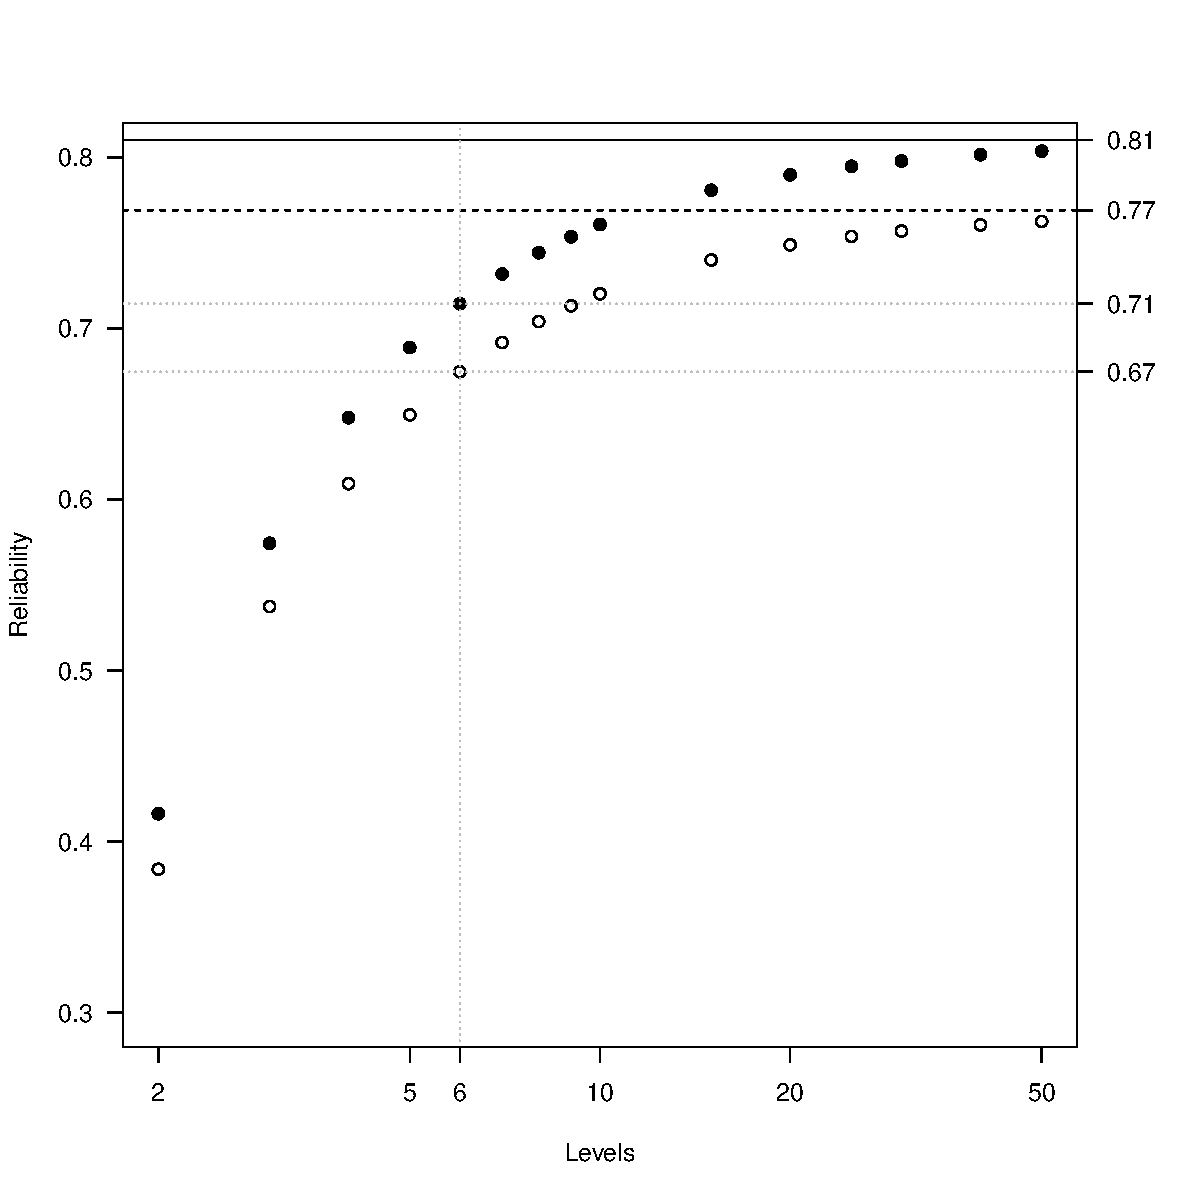
\includegraphics[scale=0.5]{chunks/ordinals}
\par\end{centering}
\caption{\label{fig:Ordinal reliability}Concrete ordinal reliability ($\fullmoon$)
and concrete ordinal \textit{H} ($\newmoon$) for a selection of Likert levels. The
theoretical coefficient $H$ is $0.81$ (solid line), and the theoretical
composite reliability is $0.77$ (dashed line). All cutoffs are uniform,
and every reliability has been calculated with $\lambda=(0.43,0.71,0.80,0.52,0.67)$
and $\sigma=(0.90,0.70,0.59,0.86,0.74)$. The original number of levels
($6$) and their corresponding concrete ordinal reliabilities $( R'_{H}=0.71, R'=0.67)$
are marked for convenience. Notice the logarithmic $x$-axis.}
\end{figure}
\begin{example}
We will yet again have a look at $6$-level agreeableness factor the
personally data $\mathtt{bfi}$ from $\mathtt{psychTools}$. The calculations in this example were done with \citep{conogive}. This package employs the $\mathtt{psych}$ \citep{psych} to fit the congeneric normal-ogive
model \eqref{eq:discretization model}. First it uses the two-step procedure
to estimate the polychoric correlation matrix, then it calls the $\mathtt{fa}$ function to run a factor analysis on the said matrix.
The resulting estimates are 
\begin{eqnarray*}
\hat{\lambda} & = & (0.43,0.71,0.80,0.52,0.67),\\
\hat{\sigma} & = & (0.90,0.70,0.59,0.86,0.74).
\end{eqnarray*} The concrete ordinal reliability
with optimal weights is $\hat{R}'_{H}=0.68$, and with equal weights
it is $\hat{R}'=0.64$. But the theoretical ordinal H is $0.81$ 
and the theoretical ordinal congeneric reliability is $0.77$ both missed by large margin. In comparison, the
reliabilities calculated under the congeneric model with $\mathtt{lavaan}$ \citep{Rosseel2012-yg}
equals $\hat{R}_{H}=0.72$, $\hat{R}=0.71$, and $\hat{R}_S = 0.72$, while $\hat{\alpha} = 0.70$ and $\hat{\alpha}_S = 0.71$.

Figure \ref{fig:Ordinal reliability} contains the calculated $ R'_{H}$ and $ R'$ for selection of Likert
scales with $\hat{\lambda} = \lambda$ and $\hat{\sigma}=\sigma$ and
the thresholds $\tau$ at $\{F^{-1}[i/(k+1)]\}_{i=1}^{k+1}$, where $F^{-1}$ is the quantile function of a standard normal. This
approximates the reliabilities we would have obtained had we used
$k+1$ Likert levels. The difference between the concrete ordinal congeneric reliability and the concrete ordinal \textit{H} is approximately $0.04$ for all $k$, but it is unclear if this relationship can be expected in other examples.

The distance from theoretical ordinal reliability to the concrete is unacceptably large when the number of Likert levels is less than or equal to $6$, where it equals about $0.1$ for both reliabilities. 
\end{example}


\section{Conclusion}
The definition of reliability \eqref{defn:reliability} entails a strong dependence between the predictor $\hat{Z}$ and the reliability coefficient $ R$. In particular, using standardized reliability \eqref{eq:Standardized reliability} is only justified if $\hat{Z}$ is the standardized score. But since the standardized score should not be used, standardized reliability should not be used either.

\citet{McNeish2019-ea} uses similar arguments against sum-scores, and makes a strong case for $ R_H$, the coefficient \textit{H}. \Cref{sec:argument B} introduced the sigma-reliability $ R_\sigma$, and similar arguments can be made against that one too: Why bother with $ R_\sigma$ when $ R_H$ is superior by definition? The main point of $ R_\sigma$ is to give $ R_H$ skeptics an alternative to standardized reliability and congeneric reliability, and \cref{thm:Properties of three} shows that $ R_\sigma$ is superior to both. 

The concrete ordinal reliability (\cref{defn:concrete ordinal reliability}) takes the dependence between reliabilities and predictors even further. This newly proposed reliability arguably measures what it should measure; how well can we predict a latent variable $Z$ given our observed data? On the other hand, the theoretical ordinal alpha only measures how well we can predict $Z$ given unobserved data. The difference between the concrete ordinal reliability and the theoretical ordinal reliability is larger than $0.1$ in our example with six Likert levels. This difference is significant and should not be ignored.

\section{Acknowledgements}
I am grateful to Riccardo De Bin and Kjersti Moss for helping me with the presentation of the paper. I am grateful to Jonas Christoffer Lindstrøm and Steffen Grønneberg for our discussions about reliability coefficients and psychometrics that inspired this paper.

\clearpage
\section*{Appendix 1: Proofs}
\label{Appendix 1}

\begin{proof}[Proof of \cref{lem:r^2 and correlation}]\label{proof:r^2 and correlation}
Recenter $Y$ and $\hat{Y}$ so that $E(Y)=E(\hat{Y})=0$. Then $\MSE(\alpha+\beta\hat{Y})$ equals $\beta^{2}\Var(\hat{Y})-2\beta\Cov(\hat{Y},Y)+\Var Y^{2}$.
Differentiate with respect to $\beta$ and set equal to zero, so that
$2\beta\Var(\hat{Y})-2\Cov(\hat{Y},Y)=0$, which implies $\beta=\Cov(\hat{Y},Y)/\Var(\hat{Y})$. Plug the expression of $\beta$ into the expression for the $\MSE$ to get \cref{eq:rsq and correlation}.
\end{proof}

\begin{proof}[Proof of Proposition \ref{prop:reliability motivation}]\label{proof:reliability motivation}
Since $\Var Z=1$, the covariance between $\hat{Z}$ and $Z$
is
\begin{equation}
\Cov(Z,\hat{Z})=\Cov[Z,{\textstyle\tsum_{i=1}^{k}w_{i}}(Z\lambda_{i}+\sigma_{i}\varepsilon)]  =  {\textstyle\tsum_{i=1}^{k}w_{i}}\lambda_{i},
\end{equation}
and the variance of $\hat{Z}$ is
\[
\Var(\hat{Z})=\Var[{\textstyle\tsum_{i=1}^{k}}w_{i}(Z\lambda_{i}+\sigma_{i}\varepsilon)]
=({\textstyle\tsum_{i=1}^{k}}w_{i}\lambda_{i})^{2}+\tsum_{i=1}^{k}w_{i}^{2}\sigma_{i}^{2}.
\]
Combining these two formulas gives us the squared correlation between
$Z$ and $\hat{Z}$,
\begin{equation}
 R_w=\Cor^{2}(\hat{Z},Z) = \frac{(\tsum_{i=1}^{k}w_{i}\lambda_{i})^{2}}{(\tsum_{i=1}^{k}w_{i}\lambda_{i})^{2}+\tsum_{i=1}^{k}w_{i}^{2}\sigma_{i}^{2}}.
\end{equation}

The second inequality is an application of \cref{lem:r^2 and correlation}.

The formula for $w_0$ follows from
\begin{equation*}
E\{[Z-\tsum_{i=1}^{k}w_{0}w_{i}(\lambda_{i}Z+\sigma_{i}\varepsilon_{i})]^{2}\} = w_{0}^{2}\tsum_{i=1}^{k}w_{i}^{2}\sigma_{i}^{2}+(w_{0}\tsum_{i=1}^{k}w_{i}\lambda_{i}-1)^{2}.
\end{equation*}
Differentiate with respect to $w_{0}$ to find the minimizer
\[
w_{0}=\frac{\tsum_{i=1}^{k}w_{i}\lambda_{i}}{(\tsum_{i=1}^{k}w_{i}^{2}\sigma_{i}^{2}+(\tsum_{i=1}^{k}w_{i}\lambda_{i})^{2})}.
\]
\end{proof}


\begin{proof}[Proof of Proposition \ref{prop:weighted alpha}]
\label{proof:weighted alpha}Clearly $wX$ is $\tau$-equivalent
if and only if $w_{i}\lambda_{i}=w_{j}\lambda_{j}$ for each $i,j$,
which implies $w^{T}\lambda=k\lambda_{i}w_{i}$. Then
\begin{eqnarray*}
\alpha_{w} & = & \frac{k}{k-1}\left(1-\frac{w^{T}\diag\Sigma w}{w^{T}\Sigma w}\right)\\
 & = & \frac{k}{k-1}\frac{k^{2}\lambda_{1}^{2}w_{1}^{2}-k\lambda_{1}^{2}w_{1}^{2}}{k^{2}\lambda_{1}^{2}w_{1}^{2}+\tsum_{i=1}^{k}w_{i}^{2}\sigma_{i}^{2}}\\
 & = & \frac{(w^{T}\lambda)^{2}}{(w^{T}\lambda)^{2}+w^{T}\Psi w.}
\end{eqnarray*}
The bias term for coefficient $\alpha_w$ can be derived as follows:
\begin{eqnarray*}
\alpha_{w} & = & \frac{k}{k-1}(1-\frac{w^{T}(\diag\Sigma)w}{w^{T}\Sigma w}),\\
 & = & \frac{k}{k-1}\frac{(w^{T}\lambda)^{2}-(w^{2})^{T}\lambda^{2}}{(w^{T}\lambda)^{2}+(w^{2})^{T}(\sigma^{2})},\\
 & = & \frac{k}{k-1}\frac{(w^{T}\lambda)^{2}-(w^{T}\lambda)^{2}/k+(w^{T}\lambda)^{2}/k-(w^{2})^{T}\lambda^{2}}{(w^{T}\lambda)^{2}+(w^{2})^{T}(\sigma^{2})},\\
 & = &  R_{w}-\frac{k}{k-1}\frac{(w^{2})^{T}\lambda^{2}-(w^{T}\lambda)^{2}/k}{(w^{T}\lambda)^{2}+(w^{2})^{T}(\sigma^{2})},\\
 & = &  R_{w}-\frac{k}{k-1}\frac{\overline{w^{2}\lambda^{2}}-\overline{w\lambda}^{2}}{k\overline{w\lambda}^{2}+\overline{w^{2}\sigma^{2}}}.
\end{eqnarray*}

Since $(\overline{w^{2}\lambda^{2}}-\overline{w\lambda}^{2})/(k\overline{w\lambda}^{2}+\overline{w^{2}\sigma^{2}})\geq0$
and equals $0$ if and only if all products $w_i\lambda_i$ are equal by Chebyshev's inequality, $\alpha_w= R_w$
iff all $w_i\lambda_i$ are equal and is otherwise an underestimate. 
\end{proof}

This lemma comes in handy in the proof of Proposition \ref{prop:Reliabilities.} as it allows us to use Jensen's inequality.

\begin{lem}
\label{lem:alpha_s}
Assume the congeneric model of \eqref{eq:congeneric model} and let $\alpha$ be as in \eqref{eq:Coefficient alpha} and $\alpha_S$ be as in \eqref{eq:standardized alpha}. Then $\alpha_S\geq\alpha$
if and only if
\begin{equation}
\label{eq:Alpha-alpha_s inequality}
\tsum_{i\neq j}\frac{\lambda_{i}\lambda_{j}}{\sqrt{\sigma_{i}^{2}+\lambda_{i}^{2}}\sqrt{\sigma_j^{2}+\lambda_{j}^{2}}} 
\geq
\tsum_{i\neq j}\frac{\lambda_{i}\lambda_{j}}{\tsum_{i=1}^{k}(\lambda_{i}^{2}+\sigma_{i}^{2})/k}.
\end{equation}
\end{lem}

\begin{proof}
From definition \eqref{eq:standardized alpha}
\begin{equation*}
\alpha_S = \frac{k}{k-1}\left(1-\frac{k}{\boldsymbol{1}^{T}\Phi\boldsymbol{1}}\right)\\
 = \frac{k}{k-1}\left(1-\frac{k}{\tsum_{i\neq j}\frac{\lambda_{i}\lambda_{j}}{\sqrt{\sigma_{i}^{2}+\lambda_{i}^{2}}\sqrt{\sigma_{j}^{2}+\lambda_{j}^{2}}}+k}\right)
\end{equation*}
and definition \eqref{eq:Coefficient alpha}
\begin{equation*}
\alpha = \frac{k}{k-1}\left(1-\frac{\tr\Sigma}{\boldsymbol{1}^{T}\Sigma\boldsymbol{1}}\right)\\
 = \frac{k}{k-1}\left(1-\frac{\tsum_{i=1}^{k}(\sigma_{i}^{2}+\lambda_{i}^{2})}{\tsum_{i\neq j}\lambda_{i}\lambda_{j}+\tsum_{i=1}^{k}(\sigma_{i}^{2}+\lambda_{i}^{2})}\right)
\end{equation*}
Thus $\alpha_S\geq\alpha$ if and only if
\[
\frac{k}{\tsum_{i\neq j}\frac{\lambda_{i}\lambda_{j}}{\sqrt{\sigma_{i}^{2}+\lambda_{i}^{2}}\sqrt{\sigma_{j}^{2}+\lambda_{j}^{2}}}+k}\leq\frac{\tsum_{i=1}^{k}(\sigma_{i}^{2}+\lambda_{i}^{2})}{\tsum_{i\neq j}\lambda_{i}\lambda_{j}+\tsum_{i=1}^{k}(\sigma_{i}^{2}+\lambda_{i}^{2})}
\]
which happens if and only if 
\[
\tsum_{i\neq j}\frac{\lambda_{i}\lambda_{j}}{\sqrt{\sigma_{i}^{2}+\lambda_{i}^{2}}\sqrt{\sigma_j^{2}+\lambda_{j}^{2}}}\geq\tsum_{i\neq j}\frac{\lambda_{i}\lambda_{j}}{\tsum_{i=1}^{k}(\lambda_{i}^{2}+\sigma_{i}^{2})/k}
\]
\end{proof}

\begin{proof}[Proof of Proposition \ref{prop:Reliabilities.}]\label{proof:Reliabilities.}
(i) From \cref{eq:Alpha-alpha_s inequality} and $\lambda_{i}=\lambda$
for all $i$, we need to show
\[
\tsum_{i\neq j}\frac{1}{\sqrt{\sigma_{i}^{2}+\lambda^{2}}\sqrt{\sigma_{j}^{2}+\lambda^{2}}}\geq\tsum_{i\neq j}\frac{1}{\tsum_{i=1}^{k}(\lambda^{2}+\sigma_{i}^{2})/k} =
\frac{k^2(k-1)}{\tsum_{i=1}^{k}(\lambda^{2}+\sigma_{i}^{2})}
\]
Recall Jensen's inequality \citep[Theorem 12 of Chapter 1]{Bullen2013-os}: When $f$ is convex, $E[f(X)]\geq f[E(X)]$ with equality if and only if $f$ is linear or $X$ is constant with probability $1$. 
Define the random variable $X$ with outcomes $(\sigma_{1}^{2},\ldots,\sigma_{k}^{2})$
and $P(X=\sigma_{i}^{2})=1/k$ for each $i$, and let $X'$ be identically
distributed to $X$ but independent of $X$. Define the function $f(x,y)=(x+\lambda^{2})^{-1/2}(y+\lambda^{2})^{-1/2}$.
Then $f$ is convex for any $\lambda$. Applying the expectation operator
first yields,
\begin{equation}
f(E(X,X'))=\frac{1}{\lambda^{2}+\frac{1}{k}\sum_{i=1}^{k}\sigma_{i}^{2}}=\frac{k}{\sum_{i=1}^{k}(\sigma_{i}^{2}+\lambda^{2})},\label{eq:f(E(X)E(X'))}
\end{equation}
while applying $f$ first yields
\begin{equation}
E(f(X,X')) = \frac{1}{k^{2}}\sum_{i\neq j}\frac{1}{(\sigma_{i}^{2}+\lambda^{2})^{1/2}(\sigma_{j}^{2}+\lambda^{2})^{1/2}}+\frac{1}{k^{2}}\sum_{i=1}^{k}\frac{1}{\sigma_{i}^{2}+\lambda^{2}}.\label{eq:E(f(XX'))}
\end{equation}
Using Jensen's inequality on \cref{eq:f(E(X)E(X'))} and \cref{eq:E(f(XX'))}
gives us
\begin{equation*}
\frac{1}{k}\sum_{i\neq j}\frac{1}{(\sigma_{i}+\lambda^{2})^{1/2}(\sigma_{j}+\lambda^{2})^{1/2}} \geq k\frac{k}{\sum_{i=1}^{k}(\sigma_{i}^{2}+\lambda^{2})}-\frac{1}{k}\sum_{i=1}^{k}\frac{1}{\sigma_{i}^{2}+\lambda^{2}}.
\end{equation*}
By the harmonic mean--arithmetic mean inequality, 
\[
\frac{1}{k}\sum_{i=1}^{k}\frac{1}{\sigma_{i}^{2}+\lambda^{2}}\geq\frac{k}{\sum_{i=1}^{k}(\sigma_{i}^{2}+\lambda^{2})},
\]
with equality if and only if all $\sigma_{i}$s are equal. Hence
\[
\sum_{i\neq j}\frac{1}{(\sigma_{i}+\lambda^{2})^{1/2}(\sigma_{j}+\lambda^{2})^{1/2}}\geq\frac{k^{2}(k-1)}{\sum_{i=1}^{k}(\sigma_{i}^{2}+\lambda^{2})},
\]
with equality if and only if all $\sigma_{i}$s are equal.

(ii) Let $k=2$. Then \eqref{eq:Alpha-alpha_s inequality} simplifies to
\[
\frac{1}{\frac{\lambda_{1}\lambda_{2}}{\sqrt{(\sigma_{1}^{2}+\lambda_{1}^{2})(\sigma_{2}^{2}+\lambda_{2}^{2})}}+1}\leq\frac{(\lambda_{1}^{2}+\sigma_{1}^{2})+(\lambda_{2}^{2}+\sigma_{2}^{2})}{2\lambda_{1}\lambda_{2}+(\lambda_{1}^{2}+\sigma_{1}^{2})+(\lambda_{2}^{2}+\sigma_{2}^{2})}
\]
and further to
\begin{equation*}
\frac{\sqrt{(\sigma_{1}^{2}+\lambda_{1}^{2})(\sigma_{2}^{2}+\lambda_{2}^{2})}}{\lambda_{1}\lambda_{2}+\sqrt{(\sigma_{1}^{2}+\lambda_{1}^{2})(\sigma_{2}^{2}+\lambda_{2}^{2})}} \geq \frac{[(\lambda_{1}^{2}+\sigma_{1}^{2})+(\lambda_{2}^{2}+\sigma_{2}^{2})]/2}{\lambda_{1}\lambda_{2}+[(\lambda_{1}^{2}+\sigma_{1}^{2})+(\lambda_{2}^{2}+\sigma_{2}^{2})]/2}
\end{equation*}
By the arithmetic mean--geometric mean inequality, $1/2[(\lambda_{1}^{2}+\sigma_{1}^{2})+(\lambda_{2}^{2}+\sigma_{2}^{2})]\geq\sqrt{(\sigma_{1}^{2}+\lambda_{1}^{2})(\sigma_{2}^{2}+\lambda_{2}^{2})}$
with equality only if $\lambda_{1}^{2}+\sigma_{1}^{2}=\lambda_{2}^{2}+\sigma_{2}^{2}$.

Let $k>2$ and assume all $\lambda_{j}=0$
except $\lambda_{1},\lambda_{2}$. By \eqref{eq:Alpha-alpha_s inequality}, $\alpha_S > \alpha$ if and
only if
\[
\frac{k}{2\frac{\lambda_{1}\lambda_{2}}{\sqrt{\sigma_{1}^{2}+\lambda_{1}^{2}}\sqrt{\sigma_{1}^{2}+\lambda_{2}^{2}}}+k}<\frac{\lambda_1^2 + \lambda_2^2 + \tsum_{i=1}^{k}\sigma_{i}^{2}}{2\lambda_{1}\lambda_{2}+\lambda_1^2 + \lambda_2^2 + \tsum_{i=1}^{k}\sigma_{i}^{2}},
\]
or, equivalently,
\begin{equation*}
\frac{k\sqrt{\sigma_{1}^{2}+\lambda_{1}^{2}}\sqrt{\sigma_{1}^{2}+\lambda_{2}^{2}}}{2\lambda_{1}\lambda_{2}+k\sqrt{\sigma_{1}^{2}+\lambda_{1}^{2}}\sqrt{\sigma_{1}^{2}+\lambda_{2}^{2}}} < \frac{\lambda_1^2 + \lambda_2^2 + \tsum_{i=1}^{k}\sigma_{i}^{2}}{2\lambda_{1}\lambda_{2}+\lambda_1^2 + \lambda_2^2 + \tsum_{i=1}^{k}\sigma_{i}^{2}},
\end{equation*}
Now, $k\sqrt{\sigma_{1}^{2}+\lambda_{1}^{2}}\sqrt{\sigma_{1}^{2}+\lambda_{2}^{2}}>\lambda_1^2 + \lambda_2^2 + \tsum_{i=1}^{k}\sigma_{i}^{2}$
can be made true by choosing $\sigma_{i}^{2}=0$ (or very small) for $i>2$ and choosing a large $k$. For the
other way around, just choose $\sigma_{i}^{2}$ large enough.

(iii) 
Observe that $\alpha_{S}\geq R$ if
and only if 
\begin{equation}
\frac{k}{k-1}\left(1-\frac{k}{\sum_{i\neq j}\frac{\lambda_{i}\lambda_{j}}{(\sigma_{i}^{2}+\lambda_{i}^{2})^{1/2}(\sigma_{i}^{2}+\lambda_{j}^{2})^{1/2}}+k}\right)\leq\frac{(\sum_{i=1}^{k}\lambda_{i})^{2}}{(\sum_{i=1}^{k}\lambda_{i})^{2}+\sum_{i=1}^{k}\sigma_{i}^{2}}.\label{eq:alpha-and-omega}
\end{equation}
Now we show that $\alpha_{S}> R$ is possible. First assume that
$\lambda_{i}=\sigma_{i}$ for each $i$. Then 
\[
\frac{\lambda_{i}\lambda_{j}}{(\sigma_{i}^{2}+\lambda_{i}^{2})^{1/2}(\sigma_{i}^{2}+\lambda_{j}^{2})^{1/2}}=\frac{\lambda_{i}\lambda_{j}}{2\lambda_{i}\lambda_{j}}=\frac{1}{2},
\]
and the left hand side of \cref{eq:alpha-and-omega} equals
\[
\frac{k}{k-1}\left(1-\frac{2}{(k+1)}\right)=\frac{k}{k+1}=\frac{1}{1+1/k}.
\]
On the other hand, the right hand side becomes
\[
\frac{(\sum_{i=1}^{k}\lambda_{i})^{2}}{(\sum_{i=1}^{k}\lambda_{i})^{2}+\sum_{i=1}^{k}\lambda_{i}^{2}}=\left(1+\frac{\sum_{i=1}^{k}\lambda_{i}^{2}}{(\sum_{i=1}^{k}\lambda_{i})^{2}}\right)^{-1}.
\]
By Chebyshev's inequality, $k\sum_{i=1}^{k}\lambda_{i}^{2}\geq(\sum_{i=1}^{k}\lambda_{i})^{2}$,
hence $(\sum_{i=1}^{k}\lambda_{i}^{2})/(\sum_{i=1}^{k}\lambda_{i})^{2}\geq1/k$
with equality if and only if all $\lambda_{i}$s are equal. It follows
that $\alpha_{S}\geq R$, with strict inequality when the $\lambda_{i}$s
are unequal.

Now we show that $\alpha_{S}\leq R$ is possible. Assume there
is an $a$ such that $\sigma_{i}^{2}+\lambda_{i}^{2}=a$ for all $i$,
that is, $\sigma_{i}^{2}+\lambda_{i}^{2}$ is constant. In this case,
\cref{eq:alpha-and-omega} becomes
\[
\frac{k}{k-1}\left(1-\frac{ak}{\sum_{i\neq j}\lambda_{i}\lambda_{j}+ak}\right)\leq\frac{(\sum_{i=1}^{k}\lambda_{i})^{2}}{\sum_{i\neq j}\lambda_{i}\lambda_{j}+ak},
\]
which can be further reduced to
\[
\frac{k}{k-1}\frac{\sum_{i\neq j}\lambda_{i}\lambda_{j}}{\sum_{i\neq j}\lambda_{i}\lambda_{j}+ak}\leq\frac{\sum_{i\neq j}\lambda_{i}\lambda_{j}+\sum_{i=1}^{k}\lambda_{i}^{2}}{\sum_{i\neq j}\lambda_{i}\lambda_{j}+ak}.
\]
This inequality is true if $(\sum_{i=1}^{k}\lambda_{i})^{2}\leq k\sum_{i=1}^{k}\lambda_{i}^{2}$,
which always holds by Chebyshev's inequality, with equality only if
all $\lambda$s are equal.

That $\alpha_{S}= R$ is possible when some $\lambda$s fail to
be equal follows from the intermediate value theorem. 
Let $A=\{ (\lambda, R)\mid\lambda_{i}\neq\lambda_{j}\text{\textrm{ for some }}j\} $.
Then $A$ is connected, and by the intermediate value theorem there
is a $(\lambda, R)$ where $[\alpha_S- R](\lambda,\sigma)=0$,
for there are elements in $A$ where $\alpha_S- R$ takes on
negative values and elements where $\alpha_S- R$ takes on positive
values.
\end{proof}

\begin{proof}[Proof of Theorem \ref{thm:ML}]\label{proof:ML}
(i) Assume the parallel model. Define $\psi^{2}$ and $\rho$ by
$\sigma^{2}+\lambda^{2}=\psi^{2}$ and $\lambda^{2}=\psi^{2}\rho$.
Then, by exercise 3.9 of \citet[][p. 114]{Muirhead2009-kq}, the maximum likelihood estimates of $\hat{\psi}^{2}$
and $\hat{\rho}$ (\citet[][Section B]{Kristof1963-tb} also worked at the maximum likelihood estimator of$\rho$) are
\[
\hat{\psi}^{2}=\tr S/k,\quad\hat{\rho}=\frac{\boldsymbol{1}^{T}S\boldsymbol{1}-\tr S}{(k-1)\tr S}1\{\boldsymbol{1}^{T}S\boldsymbol{1}\geq\tr S\}.
\]
That $\hat{\rho}=0$ when $\boldsymbol{1}^{T}S\boldsymbol{1}<\tr S$
is not explicitly stated in the exercise, but is required since $\rho\geq0$
is needed for $\Sigma$ to be positive definite. We find, using the invariance
principle for maximum likelihood,
\[
\hat{\lambda}^{2} = \frac{\boldsymbol{1}^{T}S\boldsymbol{1}-\tr S}{k(k-1)}1\{\boldsymbol{1}^{T}S\boldsymbol{1}\geq\tr S\}.
\]
Assume $\boldsymbol{1}^{T}S\boldsymbol{1}<\tr S$. Then $\hat{\sigma}^{2}=\hat{\psi}^{2}=\tr S/k$,
as claimed in the statement of this theorem. If $\boldsymbol{1}^{T}S\boldsymbol{1}\geq\tr S$,
\begin{equation*}
\hat{\sigma}^{2} = \hat{\psi}^{2}(1-\hat{\rho})
 = \frac{\tr S}{k}\left(1-\frac{\boldsymbol{1}^{T}S\boldsymbol{1}-\tr S}{(k-1)\tr S}\right)
 = \frac{\tr S-\boldsymbol{1}^{T}S\boldsymbol{1}/k}{(k-1)}.
\end{equation*}
As for (ii), first assume that $\hat{\lambda}^2\neq 0$. By the invariance property of maximum likelihood and the definition of the congeneric reliability of \cref{eq:Congeneric reliability}, the maximum likelihood estimator of the congeneric reliability is
\begin{eqnarray*}
\frac{(\boldsymbol{1}^{T}\mathbf{\hat{\lambda}})^{2}}{(\boldsymbol{1}^{T}\mathbf{\hat{\lambda}})^{2}+\boldsymbol{1}^{T}\Psi\boldsymbol{1}} & = & \frac{k(\boldsymbol{1}^{T}S\boldsymbol{1}-\textrm{tr}S)}{k(\boldsymbol{1}^{T}S\boldsymbol{1}-\textrm{tr}S)+(k\textrm{tr}S-\boldsymbol{1}^{T}S\boldsymbol{1})},\\
 & = & \frac{k(\boldsymbol{1}^{T}S\boldsymbol{1}-\textrm{tr}S)}{(k-1)\boldsymbol{1}^{T}S\boldsymbol{1}},\\
 & = & \frac{k}{k-1}\left(1-\frac{\textrm{tr}S}{\boldsymbol{1}^{T}S\boldsymbol{1}}\right).
\end{eqnarray*}
If the maximum likelihood estimator of $\lambda^{2}$ is $0$, then $(\boldsymbol{1}^{T}\mathbf{\hat{\lambda}})^{2}=0$,
and consequently the maximum likelihood estimator of the reliability is $0.$
\end{proof}

\begin{proof}[Proof of Theorem \ref{thm:asymptotics}]\label{proof:asymptotics}
(i) Let $R_{n}$, $S_{n}$ be the sample correlation and covariance matrices
and $\Phi$, $\Sigma$ be their population counterparts. By the Law
of Large Numbers and Slutsky's theorom \citep[][Lemma 2.8, p. 11]{Van_der_Vaart2000-qc}, $R_{n}\to\Phi$ and $S_{n}\to\Sigma$
with probability $1$ in the entry-wise matrix norm $\left\Vert A\right\Vert _{1}=\tsum_{j=1}^{k}\tsum_{i=1}^{k}\left|a_{ij}\right|$.
The mapping
\[
f(A)=\frac{k}{k-1}\left(1-\frac{\boldsymbol{1}^{T}(\diag A)\boldsymbol{1}}{\boldsymbol{1}^{T}A\boldsymbol{1}}\right)
\]
is continuous with respect to the norm $\left\Vert \cdot\right\Vert _{1}$,
and by the continuous mapping theorem \citep[][Theorem 2.3, p. 7]{Van_der_Vaart2000-qc} we have
$f(S_{n})\to f(\Sigma)$ and $f(R_{n})\to f(\Phi)$
with probability 1.

(ii) See Appendix 2 (p. \pageref{Appendix 2}).

(iii) \citet[eq. 22]{Van_Zyl2000-si} showed that the asymptotic variance
is
\[
\sigma^{2}(\alpha)=\frac{2k}{(k-1)[1+\rho(k-1)]^{3}}[(k-1)\rho^{3}-(2k-3)\rho^{2}+(k-3)\rho+1].
\]
This can be simplified to
\[
\sigma^{2}(\alpha)=\frac{2k(\rho-1)^{2}}{(k-1)[1+\rho(k-1)]^{2}}.
\]
\citet[equation 10]{hayashi2005note} found the asymptotic variance
\[
\sigma^{2}(\alpha_S)=\frac{1}{(k-1)^{2}}\frac{1}{(1+\rho(k-1))^{4}}2\boldsymbol{1}^{T}Q_{p}(P\otimes P)Q_{P}^{T}\boldsymbol{1}.
\]
The expression $2\boldsymbol{1}^{T}Q_{p}(P\otimes P)Q_{P}^{T}\boldsymbol{1}$
can be rewritten to \citep[Appendix 3]{hayashi2005note}
\[
2k(k-1)\{ (k-1)^{2}\rho^{4}-2(k-1)(k-2)\rho^{3}+(k^{2}-6k+6)\text{\ensuremath{\rho^{2}+2(k-2)\rho+1}}\},
\]
which can be further simplified to $(\rho-1)^{2}(1+\rho(k-1)^{2})^{2}$.
Thus
\[
\sigma^{2}(\alpha_S)=\frac{2k}{(k-1)}\frac{2k(\rho-1)^{2}}{(k-1)[1+\rho(k-1)]^{2}},
\]
and the limits are equal.

Since
\begin{equation*}
\alpha_S = \frac{k}{k-1}\left(1-\frac{k}{k(k-1)\rho+k}\right) = \frac{k\rho}{(k-1)\rho+1},
\end{equation*}
we get that $1-\alpha_S = (1-\rho)/((k-1)\rho+1)$. Taken together, the asymptotic variance is
\[
\sigma^{2}(\alpha_S)=2\frac{k}{k-1}(1-\alpha_S)^{2}.
\]
Since $\hat{\alpha}$ is the maximum likelihood estimator of $ R$
when $n$ is large it is efficient. And since the asymptotic variances
of $\hat{\alpha}$ and $\hat{\alpha_S}$ coincide they
are both efficient.
\end{proof}

The proof of \cref{thm:Properties of three} uses the theory of power means. Let $p$ be real number and $x=\{x_{i}\} _{i=1}^{k}$ be a sequence
of positive reals. The \textit{power mean} with exponent $p$ is
\[
M_{p}(x)=\begin{cases}
(\frac{1}{k}\tsum_{i=1}^{k}x_{i}^{p})^{1/p} & p\neq0,\\
(\prod_{i=1}^{k}x_{i})^{1/k} & p=0.
\end{cases}
\]
We will make use of a generalization of the arithmetic mean--geometric mean and harmonic mean--arithmetic mean inequalities. The \textit{power mean inequality} \citep[][Chapter III]{Bullen2013-os} is
\begin{equation}
M_{p}(x)\leq M_{q}(x),\quad p<q\label{eq:generalized mean inequality}
\end{equation}
with equality if and only if $x_{1}=\cdots=x_{k}$. 

Moreover, a generalized Minkowski inequality holds for the power means. See \citep[][Section 2.4, Theorem 9.]{Bullen2013-os} for proofs of this result.

\begin{thm}[Minkowski inequality]
\label{thm:minkowski}
Let $x,y$ be $k$-ary sequences of non-negative reals. Then
\begin{align}
M_{p}^{p}(x)+M_{p}^{p}(y) & \geq M_{p}^{p}(x+y),\;p>1,\label{eq:Minkowski 1}\\
M_{p}(x)+M_{p}(y) & =M_{1}(x+y),\;p=1,\label{eq:Minkowski 2}\\
M_{p}^{p}(x)+M_{p}^{p}(y) & \leq M_{p}^{p}(x+y),\;p<1.\label{eq:Minkowski 3}
\end{align}
Here \cref{eq:Minkowski 1} and \cref{eq:Minkowski 3} are equalities if and only there are some $\lambda,\mu\in\mathbb{R}$,
not both $0$, such that $\lambda x+\mu y=0$.
\end{thm}
This lemma is instrumental to the proof of \cref{thm:Properties of three}.
\begin{lem}
\label{lem:power mean lemma}Let $\{ x_{i}\} _{i=1}^{k}$
be some positive real numbers, $a>0$, and $M_{p}(x)$
the power mean with exponent $p$. 
\begin{equation}
M_{p}(x+a)M_{q}(x/{(x+a)})\leq\overline{x}\label{eq:power mean inequality}
\end{equation}
when $p,q\leq1$, with equality if and only if $x_{1}=x_{2}=\cdots=x_{k}$.
If $-1\leq p<0$, 
\begin{equation}
M_{p}(x)\leq M_{p}(x+a)M_{p}(x/{(x+a)})\leq\overline{x}\label{eq:power mean full inequality}
\end{equation}
holds too, again with equality if and only if $x_{1}=x_{2}=\cdots=x_{k}$.
\end{lem}
\begin{proof}
Consider \cref{eq:power mean inequality} first. By the power
mean inequality (\cref{eq:generalized mean inequality}) we have $M_{p}(x+a)\leq\overline{x}+a$ and $M_{q}(x/(x+a))\leq\overline{x/(x+a)}$,
hence it suffices to show $(\overline{x}+a)\overline{x/(x+a)}\leq\overline{x}$,
or equivalently, $\overline{x/(x+a)}\leq\overline{x}/(\overline{x}+a)$.
The function $x\mapsto x/(a+x)$ is concave, hence $E[f(X)]\leq f[E(X)]$
by Jensen's inequality. But then $\overline{x/(x+a)}\leq\overline{x}/(\overline{x}+a)$
follows.

Now let us take on \cref{eq:power mean full inequality}.
Since $-1\leq p<0$, the function $f(x)=x^{p}/(x^{p}+a)$ is convex, as can
be verified by differentation. Hence $f(E(x))\leq Ef(x)$ by Jensen's
inequality (here $x$ is regarded as a uniform random variable). Since
\[
E[f(x)]=k^{-1}\tsum_{i=1}^{k}x_{i}^{p}/(x_{i}^{p}+a)=M_{p}^{p}(x/(x+a)),
\]
and
\[
f[E(x)]=\overline{x^{p}}/(\overline{x^{p}}+a)=M_{p}^{p}(x)/(M_{p}^{p}(x)+a),
\]
we get that $M_{p}^{p}(x)/[M_{p}^{p}(x)+a]\leq M_{p}^{p}(x/(x+a)$. Moreover, $M_{p}^{p}(x)+a=M_{p}^{p}(x)+M_{p}^{p}(a)\leq M_{p}^{p}(x+a)$
by the Minkowski inequality (\cref{eq:Minkowski 3}), hence $M_{p}(x)/M_{p}(x+a)\leq M_{p}(x/(x+a))$. This can be rearranged to get the left-most inequality. 
Now notice that the right-most inequality is a special case of \cref{eq:power mean inequality}, and we are done. 
\end{proof}

\begin{proof}[Proof of \cref{thm:Properties of three}]
\label{proof:Properties}
(i) The equality $ R_H \geq  R_\sigma$ trivially true, so we will focus on the rest. Each reliability is on the form $a/(a+1)$ for some $a>0$, and $a/(a+1)\geq b/(b+1)$
iff $a>b$. Let's take on $ R_S >  R$. From \cref{eq:Congeneric reliability} and \cref{eq:Standardized reliability} we see that we must verify
\[
k\overline{\lambda(\lambda^{2}+\sigma^{2})^{-1/2}}^{2}/\overline{\sigma^{2}(\lambda^{2}+\sigma^{2})^{-1}}\geq k\overline{\lambda}^{2}/\overline{\sigma^{2}}.
\]
Since all $\lambda_i$s are equal by assumption, this is equivalent to 
\[
\overline{\sigma^{2}/(\lambda^{2}+\sigma^{2})}/\overline{(\lambda^{2}+\sigma^{2})^{-1/2}}^{2}\leq\overline{\sigma^{2}}
\]
which is true by Lemma \ref{lem:power mean lemma}, \cref{eq:power mean inequality} using exponent $p = -1/2$, $q = 1$ and $a = \lambda^2$.

To prove $ R_{\sigma}> R_{S}$, refer to \cref{eq:Sigma-standardized reliability} and \cref{eq:Standardized reliability} to verify that we need to show
\[
\overline{\sigma^{-1}}^{-2}\leq\overline{\sigma^{2}/(\lambda^{2}+\sigma^{2})}/\overline{(\lambda^{2}+\sigma^{2})^{-1/2}}^{2},
\]
or equivalently,
\[
M_{-1/2}(\sigma^{2})\leq \overline{\sigma^{2}/\lambda^{2}+\sigma^{2}}M_{-1/2}(\lambda^{2}+\sigma^{2}).
\]
This is a case of \cref{lem:power mean lemma}, \cref{eq:power mean full inequality}, as $\overline{\sigma^{2}/\lambda^{2}+\sigma^{2}} \geq M_{-1/2}(\sigma^{2}/\lambda^{2}+\sigma^{2})$ by the power mean inequality.

(ii) That $R_{\sigma}=R$ follows from \cref{prop:reliability motivation}, and $R_{H}\geq R_{\sigma}$
since the weights of $R_{H}$ are optimal. It suffices to show $R\geq R_{S}$.
From the proof of (i), we must verify
\[
\overline{\sigma^{2}(\lambda^{2}+\sigma^{2})}/\overline{(\lambda^{2}+\sigma^{2})^{-1/2}}^{2}\geq\sigma^{2}
\]
Since $\overline{\sigma^{2}(\lambda^{2}+\sigma^{2})}=\sigma^{2}\overline{(\lambda^{2}+\sigma^{2})}$,
this is equivalent to
\[
\overline{(\lambda^{2}+\sigma^{2})}\geq\overline{(\lambda^{2}+\sigma^{2})^{-1/2}}^{2},
\]
but this follows from the power mean inequality, \cref{eq:generalized mean inequality}.


\end{proof}

\begin{proof}[Proof of Theorem (\ref{thm:omega-prime})]
\label{proof:omega-prime}(ii) That $ R'=1-\MSE(v_{0}\hat{Z})$
follows from Lemma \ref{lem:r^2 and correlation} and the formula
for the covariance, which we now show. By the law of total covariance, the covariance between $\tsum_{i=1}^{k}w_{i}\hat{X}_{i}$
and $Z$ is
\begin{eqnarray*}
\Cov(\tsum_{i=1}^{k}w_{i}\hat{X}_{i},Z) & = & E[\Cov(\tsum_{i=1}^{k}w_{i}\hat{X}_{i},Z\mid\{Y_{i}\})]+\Cov(E[\tsum_{i=1}^{k}w_{i}\hat{X}_{i}\mid\{Y_{i}\}],E[Z\mid\{Y_{i}\}]),\\
 & = & \Cov(\tsum_{i=1}^{k}w_{i}\hat{X}_{i},E[Z\mid\{Y_{i}\}]).
\end{eqnarray*}
The second equality holds since $\Cov(\tsum_{i=1}^{k}w_{i}\hat{X}_{i},Z\mid\{Y_{i}\}) = 0$, as $X_i$ is a constant function of $Y_i$, and $E[\tsum_{i=1}^{k}w_{i}\hat{X}_{i}| \{Y_{i}\}] = \tsum_{i=1}^{k}w_{i}\hat{X}_{i}$.
The expectation $E[Z\mid\{Y_{i}\}]$ equals $E[E[Z\mid X]\mid\{Y_{i}\}]$.
The conditional expectation $E(Z\mid X)=\tsum_{i=1}^{k}v_{i}X_{i}$
under multivariate normality, where $v_{i}=\lambda_{i}/[\sigma_{i}^{2}(1+k\overline{\lambda^{2}\sigma^{-2}})]$
are the Thurstone weights, see \citet[Theorem 3.3.4]{Tong1990-lm}.
Consequently, $E[E(Z\mid X)\mid\{Y_{i}\}]=\tsum_{i=1}^{k}v_{i}\hat{X_{i}}$
and 
\begin{equation*}
\Cov(\tsum_{i=1}^{k}w_{i}\hat{X}_{i},Z) =  \Cov(\tsum_{i=1}^{k}w_{i}\hat{X}_{i},\tsum_{i=1}^{k}v_{i}\hat{X}_{i})=w^{T}\Xi v.
\end{equation*}
Standardize to find the correlation $w^{T}\Xi v/\sqrt{w^{T}\Xi w}$,
and the squared correlation is $ R'=(w^{T}\Xi v)^{2}/w^{T}\Xi w$.
This completes point (i). 

As for (iii), under the parallel model, $v=w_{0}\boldsymbol{1}$, where
$w_{0}=\lambda/[\sigma^{2}+k\lambda^{2}]$ and the squared correlation
is $w_{0}^{2}\boldsymbol{1}^{T}\Xi\boldsymbol{1}=\lambda^{2}\boldsymbol{1}^{T}\Xi\boldsymbol{1}/(k\lambda^{2}+\sigma^{2})^{2}$.
For the second equation, first notice that
\[
\alpha_S=\frac{k}{k-1}\frac{i^{T}\Phi i-k}{i^{T}\Phi i}=k^{2}\frac{\rho}{i^{T}\Phi i},
\]
where $\overline{\rho}$ is the unique correlation. Since $(k\lambda^{2}+\sigma^{2})^{2}=(i^{T}\Phi i/k)^{2}$, 
\begin{equation}
\frac{\lambda^{2}}{(k\lambda^{2}+\sigma^{2})^{2}}\boldsymbol{1}^{T}\Xi\boldsymbol{1} =  k^{2}\frac{\rho}{(i^{T}\Phi i)^{2}}\boldsymbol{1}^{T}\Xi\boldsymbol{1} =  \alpha_S\frac{\boldsymbol{1}^{T}\Xi\boldsymbol{1}}{\boldsymbol{1}^{T}\Psi\boldsymbol{1}},\nonumber
\end{equation}
as claimed.

(i) Follows from the representation $R_w = (w^T\Xi v)^2/(w^T\Xi w)$. We use the derivatives $\frac{d}{dw}w^{T}\Xi w=2w^{T}\Xi$ and $\frac{d}{dw}w^{T}\Xi v=v^{T}\Xi$,
so that $\frac{d}{dw}(w^{T}\Xi v)^{2}=2(w^{T}\Xi v)v^{T}\Xi$. Now
apply the quotient rule
\begin{eqnarray*}
\frac{d}{dx}\frac{(x^{T}\Xi y)^{2}}{x^{T}\Xi x} & = & \frac{2(w^{T}\Xi v)v^{T}\Xi(w^{T}\Xi w)-(w^{T}\Xi v)^{2}2w^{T}\Xi}{(w^{T}\Xi w)^{2}}
\end{eqnarray*}
This is equal to $0$ when $w=v$, for $v^{T}\Xi(v^{T}\Xi v)^{2}-(v^{T}\Xi v)^{2}v^{T}\Xi=0$.
\end{proof}
%\clearpage
\section*{Appendix 2: Proof of Theorem \ref{thm:asymptotics} (ii)}
\label{Appendix 2}

In this appendix we prove a more detailed variant of Theorem \ref{thm:asymptotics} (ii).
\begin{prop}
\label{prop:equal limis}Assume the parallel model with finite fourth
moments, $k\times k$ covariance matrix $\Sigma$, variances $\phi^{2}$,
and correlation $\rho$. Then the asympotic variances of standardized
alpha and coefficient alpha are both equal to 
\begin{equation}
\sigma^{2}=\sigma_{s}^{2}=\frac{1}{(k-1)^{2}}\frac{1}{[(k-1)\rho+1]^{4}}\frac{1}{\phi^{4}}v^{T}\Gamma v,\label{eq:asymptotic variance-1}
\end{equation}
where 
\begin{equation}
\nonumber
\Gamma = E[XX^{T}\otimes XX^{T}]-(\vvec\Sigma)(\vvec\Sigma)^{T},
\end{equation}
 and
\[
v=[(k-1)\rho+1]\vvec(I_{p})-\vvec(\boldsymbol{1}\boldsymbol{1}^{T}).
\]
\end{prop}

The operation $\otimes$ denotes the Kronecker product. The proof and statement of Proposition (\ref{prop:equal limis}) makes use of three
kinds of \emph{vectorizations}, operations that map matrices into
vectors. The first operation is full vectorization, $\vvec A$, which
maps the $m\times n$ matrix $A$ to the $mn$ column vector $(A_{\cdot1},A_{\cdot2},\ldots,A_{\cdot n})$
\citep[Chapter 2.4]{Magnus2019-cz}. The second operation is half-vectoriazation,
where $\vech A$ maps the symmetric $n\times n$ matrix $A$ to the
$n(n+1)/2$ vector obtained by stacking the columns of the lower triangular
part of $A$ \citep[Chapter 3.8]{Magnus2019-cz}. The third $\w(A)$
operation maps the symmetric $n\times n$ matrix with $0$ diagonal
to the $n(n-1)/2$ vector obtained by stacking the columns of the
infradiagonal elements of $A$; that is, it the variant of half-vectorization
that ignores the main diagonal \citep{Neudecker1996-fu}. 

Define the transition matrices $L_{k}$ by $\vvec A=L_{k}^{T}\vech(A)$
and $L_{k}^{-}$ by $\vech(A)=L_{k}^{-^{T}}\vvec A$ when the $k\times k$
matrix $A$. These matrices
are called $K_{k}$ and $K_{k}^{-}$ by \citet{Van_Zyl2000-si}. The
matrix $D$ satisfies $\vvec A=D\w(A)$ and $\w(A)=\frac{1}{2}D^{T}\vvec(A)$
when $A$ is symmetric with $0$ on the diagonal \citep{Neudecker1996-fu}.
The matrix $K$ is the \emph{commutation matrix}, making $K\vvec X=\vvec X^{T}$
\citep[see][Chapter 3.8]{Magnus2019-cz}, and $K_{d}$ is the diagonal
of $K$. In general, if $A$ is a square matrix, $A_{d}$ is the matrix
with the same diagonal as $A$ and off-diagonal elements set to $0$. 
\begin{lem}
\label{lem:variances}Assume the parallel model with variance $\phi^{2}$
and correlation $\rho$, covariance matrix $\Sigma$, correlation
matrix $\Phi$. Then the asymptotic variance for coefficient alpha is as in Proposition \ref{prop:equal limis}. The asymptotic variance for standardized alpha is 
\begin{equation}
\nonumber
\sigma^{2}=\frac{1}{(k-1)^{2}}\frac{1}{[\{(k-1)\rho+1]^{4}}\frac{1}{\phi^{4}}\boldsymbol{1}_{*}^{T}D^{T}\Psi_{*}D\boldsymbol{1}_{*},
\end{equation}
where $\boldsymbol{1}_{*}$ has $\frac{1}{2}k(k-1)$ elements and
\[
\Psi_{*}=[I-(I\otimes\Phi)K_{d}]\Gamma[I-K_{d}(I\otimes\Phi)].
\]
\end{lem}

\begin{proof}
We will take coefficient alpha first. \citet{Van_Zyl2000-si} showed that, in the case
of multivariate normality, $\sigma^{2}=h^{T}L_{k}^{T}2(\Sigma\otimes\Sigma)L_{k}h$,
where $h$ is \citep[eq. 19]{Van_Zyl2000-si}
\begin{equation*}
h = (\boldsymbol{1}^{T}\Sigma\boldsymbol{1})^{-2}[(\boldsymbol{1}^{T}\Sigma\boldsymbol{1}^{T}\vvec I-\tr\Sigma\vvec(\boldsymbol{1}\boldsymbol{1}^{T})]L_{k}^{-}.
\end{equation*}
Now we use Theorem 1 of \citet{Neudecker1990-ph} to generalize the formula for $\sigma^2$ to non-normal variables; the substitution
$2(\Phi\otimes\Phi)=\Gamma$ gives the general formula $\sigma^{2}=h^{T}L_{k}^{T}\Gamma L_{k}h.$

Using the identities
\begin{eqnarray*}
\boldsymbol{1}^{T}\Sigma\boldsymbol{1} & = & \phi^{2}k\{(k-1)\rho+1,\\
\tr\Sigma & = & \phi^{2}k,
\end{eqnarray*}
we obtain
\begin{eqnarray*}
h & = & \frac{[\phi^{2}k\{(k-1)\rho+1\}]\vvec(I_{p})-\phi^{2}k\vvec(\boldsymbol{1}\boldsymbol{1}^{T})}{[\phi^{2}k\{(k-1)\rho+1]^{2}}L_{k}^{-},\\
 & = & \frac{[\{(k-1)\rho+1]\vvec(I_{p})-\vvec(\boldsymbol{1}\boldsymbol{1}^{T})}{\phi^{2}k[(k-1)\rho+1]^{2}}L_{k}^{-}.
\end{eqnarray*}
Define
\[
g=\{[(k-1)\rho+1]\vvec(I_{p})-\vvec(\boldsymbol{1}\boldsymbol{1}^{T})\}L_{k}^{-},
\]
so that
\[
\sigma^{2}=\frac{1}{(k-1)^{2}}\frac{1}{[\{(k-1)\rho+1]^{4}}\frac{1}{\phi^{4}}g^{T}L_{k}^{T}\Gamma L_{k}g.
\]
Moreover, $L_{k}L_{k}^{-}=M_{p}$, which satisifies $M_{p}\vvec S=\vvec S$
whenever $S$ is symmetric, see \citet[p. 275]{Van_Zyl2000-si}. Thus 
\begin{eqnarray*}
\sigma^{2} & = & \frac{1}{(k-1)^{2}}\frac{1}{[\{(k-1)\rho+1]^{4}}\frac{1}{\phi^{4}}v^{T}M_{p}^{T}\Gamma M_{p}^{T}v,\\
 & = & \frac{1}{(k-1)^{2}}\frac{1}{[\{(k-1)\rho+1]^{4}}\frac{1}{\phi^{4}}v^{T}\Gamma v.
\end{eqnarray*} where $v$ is defined in Proposition \ref{prop:equal limis}.

Now it is time for standardized alpha. Combining equations (8) and (9) of \citet{hayashi2005note},
we find that the asymptotic variance for standardized alpha is
\begin{equation*}
\sigma_{s}^{2}=\frac{1}{(k-1)^{2}}\left(\frac{1}{1+\rho(k-1)}\right)^{4}\boldsymbol{1}_{*}^{T}D^{T}\Psi D\boldsymbol{1}_{*},\label{eq:standardized alpha variance 3}
\end{equation*}
where 
\[
\Psi=[I-(I\otimes\Phi)K_{d}](\Sigma_{d}^{-1/2}\otimes\Sigma_{d}^{-12})\Gamma(\Sigma_{d}^{-1/2}\otimes\Sigma_{d}^{-12})[I-K_{d}(I\otimes\Phi)]
\]
Since $\Sigma_{d}^{-1/2}=\phi^{-1}I$,
\[
\Sigma_{d}^{-1/2}\otimes\Sigma_{d}^{-12}=\phi^{-1}I\otimes\phi^{-1}I=\phi^{-2}I\otimes I=\phi^{-2}I.
\]
hence 
\[
\Psi=\phi^{-4}[I-(I\otimes\Phi)K_{d}]\Gamma[I-K_{d}(I\otimes\Phi)].
\]
\end{proof}

Propositon \ref{prop:equal limis} now follows from this lemma.
\begin{lem}
The following equalities are true
\begin{equation*}
 \{I-K_{d}(I\otimes \Phi)\}D\boldsymbol{1}_{*}
= \{I-K_{d}(I\otimes \Phi)\}[\vvec(\boldsymbol{1}\boldsymbol{1}^{T})-\vvec I]
= \vvec(\boldsymbol{1}\boldsymbol{1}^{T})-[(k-1)\rho+1]\vvec(I_{p}).
\end{equation*}
\end{lem}

\begin{proof}
First observe that $D\boldsymbol{1}_{*}=\vvec(\boldsymbol{1}\boldsymbol{1}^{T})-\vvec I$
by the definition of $D$, proving the first inequality. 

Now we show that $(I-K_{d}(I\otimes \Phi))\vvec I=0$. First observe
that $(I\otimes \Phi)\vvec I=\vvec\Phi$ by Theorem 2.2 of \citet{Magnus2019-cz}.
The operation $K_{d}\vvec A$ selects the ``diagonal'' elements
of $\vvec A$, i.e., $K_{d}\vvec A=\vvec A_{d}$. Since $\Phi_{d}=I$,
$K_{p}\vvec\Phi=K_{p}\vvec I=\vvec I$, and therefore $(I-K_{d}(I\otimes\Phi))\vvec I=0$
as claimed.

The next step is $K_{d}(I\otimes \Phi)\vvec(\boldsymbol{1}\boldsymbol{1}^{T})=(1+(k-1)\rho)\boldsymbol{1}\boldsymbol{1}^{T}$.
First, by Theorem 2.2 of \citet{Magnus2019-cz}, $K_{d}(I\otimes\Phi)\vvec(\boldsymbol{1}\boldsymbol{1}^{T})=K_{d}\vvec(\Phi\boldsymbol{1}\boldsymbol{1}^{T})$.
Since $\Phi\boldsymbol{1}\boldsymbol{1}^{T}=[1+(k-1)\rho]\boldsymbol{1}\boldsymbol{1}^{T}$,
$K_{d}\vvec(\Phi\boldsymbol{1}\boldsymbol{1}^{T})=[1+(k-1)\rho]K_{d}\vvec(\boldsymbol{1}\boldsymbol{1}^{T})$,
but since $K_{d}\vvec(\boldsymbol{1}\boldsymbol{1}^{T})=\vvec I$, we get
$K_{d}(I\otimes\Phi)\vvec(\boldsymbol{1}\boldsymbol{1}^{T})=[1+(k-1)\rho]\vvec I$.
\end{proof}

\bibliography{standardized}

\end{document}
